\documentclass[sigconf]{acmart}
\def\BibTeX{{\rm B\kern-.05em{\sc i\kern-.025em b}\kern-.08emT\kern-.1667em\lower.7ex\hbox{E}\kern-.125emX}}
    
% Rights management information. 
% This information is sent to you when you complete the rights form.
% These commands have SAMPLE values in them; it is your responsibility as an author to replace
% the commands and values with those provided to you when you complete the rights form.
%
% These commands are for a PROCEEDINGS abstract or paper.
\copyrightyear{2019}
\acmYear{2019}
\setcopyright{acmlicensed}
\acmConference[SC '19]{SC '19: The International Conference for High Performance Computing Networking, Storage, and Analysis}{November 17--22, 2019}{Denver, CO}
%\acmBooktitle{SC '19: ACM Symposium on Neural Gaze Detection, June 03--05, 2018, Woodstock, NY}
\acmPrice{15.00}
%\acmDOI{10.1145/1122445.1122456}
%\acmISBN{978-1-4503-9999-9/18/06}

\usepackage{xcolor} 
\usepackage[noend]{algpseudocode}
\usepackage{array}
\usepackage{amsfonts}
%\usepackage{graphicx}
\usepackage{epstopdf}
\usepackage{amssymb}
\usepackage{tikz,pgfplots}
\usetikzlibrary{snakes,arrows,shapes,trees}
\usepackage[position=top,aboveskip=5pt,labelformat=empty]{subfig}
%\usepackage{amssymb,amsmath,amsthm}
\usepackage{amsopn}
\usepackage{listings}
\usepackage{adjustbox}
\usepackage{longtable}
\usepackage{multirow}
\usepackage{minted}
\usepackage{amssymb}
\usepackage{pgfplots}
\usepackage{pgfplotstable}
\usetikzlibrary{arrows,shapes,plotmarks}
\pgfplotsset{compat=1.8}
\usepackage{soul}
\usepackage{rotating}
\usepackage{url}
\usepackage{algorithm}
\usepackage{enumitem}


\newcommand{\mynote}[3]{
	\textcolor{#2}{\fbox{\bfseries\sffamily\scriptsize#1}}
		{\small$\blacktriangleright$\textsf{\emph{#3}}$\blacktriangleleft$}
}

\newcommand{\bg}[1]{\mynote{Baskar}{magenta}{#1}}
\newcommand{\hs}[1]{\mynote{Hari}{olive}{#1}}
\newcommand{\ks}[1]{\mynote{Kumar}{blue}{#1}}
\newcommand{\bk}[1]{\mynote{Biswajit}{teal}{#1}}
\newcommand{\mi}[1]{\mynote{Masado}{lime}{#1}}
\newcommand{\mf}[1]{\mynote{Milinda}{brown}{#1}}

\newcommand{\stri}{sedectree} 
\newcommand{\stra}{sedecant}

\newcommand{\mvec}{\textsc{matvec}}
\newcommand{\sfcmvec}{\textsc{SFC-MATVEC}}
\newcommand{\tsort}{\textsc{TreeSort}}
\newcommand{\tsearch}{\textsc{TreeSearch}}
\newcommand{\tcons}{\textsc{TreeConstruction}}
\newcommand{\dtcons}{\textsc{DistTreeConstruction}}
\newcommand{\taux}{\textsc{AuxiliaryOctants}}
\newcommand{\tbal}{\textsc{TreeBalancing}}
\newcommand{\tdbal}{\textsc{DistTreeBalancing}}
\newcommand{\tghost}{\textsc{ComputeGhostElements}}
\newcommand{\teToe}{\textsc{BuildE2E}}
\newcommand{\teTon}{\textsc{BuildE2N}}

\newcommand{\dendrokt}{\textsc{XVI}}

\newcommand{\hilbertcurve}{\textsc{Hilbert}}
\newcommand{\mortoncurve}{\textsc{Morton}}


\newcommand{\tsortmodified}{\textsc{TreeSortModified}}
\newcommand{\dtsortmodified}{\textsc{DistTreeSortModified}}
\newcommand{\tbucket}{\textsc{SFC\_Bucketing}}
\newcommand{\maxDepth}{\textsc{maxdepth}}
%\newcommand{\tsort_cons}{\textsc{OctreeConstruction}}
\newcommand{\ssort}{\textsc{SampleSort}}
\newcommand{\dsort}{\textsc{DistTreeSort}}
\newcommand{\note}[1]{\noindent\emph{\textcolor{purple}{hs: #1}}}
%\algrenewcommand\algorithmicrequire{\textbf{Input:}}
%\algrenewcommand\algorithmicensure{\textbf{Output:}}
%\algrenewcommand\algorithmicforall{\textbf{parallel for}}

\newcommand{\Intel}{Intel\textsuperscript{\textregistered}\xspace}
\newcommand{\snb}{Xeon\texttrademark\xspace}
\newcommand{\xphi}{Xeon Phi\texttrademark\xspace}
\newcommand{\Summit}{\href{https://www.olcf.ornl.gov/summit/}{Summit}}
\newcommand{\Aurora}{\href{http://aurora.alcf.anl.gov/}{Aurora}}
\newcommand{\Stampede}{\href{https://www.tacc.utexas.edu/systems/stampede2}{Stampede2}}
\newcommand{\Titan}{\href{https://www.olcf.ornl.gov/titan/}{Titan}}
\newcommand{\petsc}{\href{https://www.mcs.anl.gov/petsc/}{PETSc}}

\newcommand{\octdomain}{\mathcal{N}^3}
%%

\newcommand{\Tau}{\mathcal{T}}

\newdimen\HilbertLastX
\newdimen\HilbertLastY
\newcounter{HilbertOrder}

\def\DrawToNext#1#2{%
  \advance \HilbertLastX by #1
  \advance \HilbertLastY by #2
  \pgfpathlineto{\pgfqpoint{\HilbertLastX}{\HilbertLastY}}
  % Alternative implementation using plot streams:
  % \pgfplotstreampoint{\pgfqpoint{\HilbertLastX}{\HilbertLastY}}
}

% \Hilbert[right_x,right_y,left_x,left_x,up_x,up_y,down_x,down_y]
\def\Hilbert[#1,#2,#3,#4,#5,#6,#7,#8] {
  \ifnum\value{HilbertOrder} > 0%
  \addtocounter{HilbertOrder}{-1}
  \Hilbert[#5,#6,#7,#8,#1,#2,#3,#4]
  \DrawToNext {#1} {#2}
  \Hilbert[#1,#2,#3,#4,#5,#6,#7,#8]
  \DrawToNext {#5} {#6}
  \Hilbert[#1,#2,#3,#4,#5,#6,#7,#8]
  \DrawToNext {#3} {#4}
  \Hilbert[#7,#8,#5,#6,#3,#4,#1,#2]
  \addtocounter{HilbertOrder}{1}
  \fi
}

% \hilbert((x,y),order)
\def\hilbert((#1,#2),#3){%
  \advance \HilbertLastX by #1
  \advance \HilbertLastY by #2
  \pgfpathmoveto{\pgfqpoint{\HilbertLastX}{\HilbertLastY}}
  % Alternative implementation using plot streams:
  % \pgfplothandlerlineto
  % \pgfplotstreamstart
  % \pgfplotstreampoint{\pgfqpoint{\HilbertLastX}{\HilbertLastY}}
  \setcounter{HilbertOrder}{#3}
  \Hilbert[1mm,0mm,-1mm,0mm,0mm,1mm,0mm,-1mm]
  \pgfusepath{stroke}%
}


\ifpdf
  \DeclareGraphicsExtensions{.eps,.pdf,.png,.jpg}
\else
  \DeclareGraphicsExtensions{.eps}
\fi

%strongly recommended
%\numberwithin{theorem}{section}

\definecolor{cpu3}{HTML}{F44336}
\definecolor{cpu4}{HTML}{2196F3}
\definecolor{cpu1}{HTML}{4CAF50}
\definecolor{cpu2}{HTML}{FFC107}
\definecolor{gpu3}{HTML}{EF9A9A}
\definecolor{gpu4}{HTML}{90CAF9}
\definecolor{gpu1}{HTML}{A5D6A7}
\definecolor{gpu2}{HTML}{FFE082}

\definecolor{cpu5}{HTML}{9932CC}

\definecolor{sq_b1}{RGB}{37,52,148}
\definecolor{sq_b2}{RGB}{44,127,184}
\definecolor{sq_b3}{RGB}{65,182,196}
\definecolor{sq_b4}{RGB}{127,205,187}
\definecolor{sq_b5}{RGB}{199,233,180}
\definecolor{sq_b6}{RGB}{255,255,204}

\definecolor{sq_r1}{RGB}{189,0,38}
\definecolor{sq_r2}{RGB}{240,59,32}
\definecolor{sq_r3}{RGB}{253,141,60}
\definecolor{sq_r4}{RGB}{254,178,76}
\definecolor{sq_r5}{RGB}{254,217,118}
\definecolor{sq_r6}{RGB}{255,255,178}

\definecolor{sq_g1}{RGB}{0,104,55}
\definecolor{sq_g2}{RGB}{49,163,84}
\definecolor{sq_g3}{RGB}{120,198,121}
\definecolor{sq_g4}{RGB}{173,221,142}
\definecolor{sq_g5}{RGB}{217,240,163}
\definecolor{sq_g6}{RGB}{255,255,204}


\definecolor{div_c1}{RGB}{230,171,2}
\definecolor{div_c2}{RGB}{102,166,30}
\definecolor{div_c3}{RGB}{231,41,138}
\definecolor{div_c4}{RGB}{117,112,179}
\definecolor{div_c5}{RGB}{217,95,2}
\definecolor{div_c6}{RGB}{27,158,119}
\definecolor{div_c7}{RGB}{215,48,39}

\definecolor{div_d1}{RGB}{215,25,28}
\definecolor{div_d2}{RGB}{253,174,97}
\definecolor{div_d3}{RGB}{255,255,191}
\definecolor{div_d4}{RGB}{171,217,233}
\definecolor{div_d5}{RGB}{44,123,182}




\definecolor{lineclr}{RGB}{0,0,0}
\definecolor{utorange}{RGB}{0,0,255}
\definecolor{utsecblue}{RGB}{255,255,0}
\definecolor{utsecgreen}{RGB}{255,0,0}
\definecolor{red!15}{RGB}{0,255,255}
\definecolor{fillclr5}{RGB}{0,255,0}
\definecolor{fillclr6}{RGB}{255,0,255}
\definecolor{fillclr7}{RGB}{255,255,255}
\definecolor{fillclr8}{RGB}{0,0,0}





\def\drawcubeI(#1,#2,#3,#4,#5){ % x,y,z,sz,line color
\coordinate (O) at (#1,#2,#3);
\coordinate (A) at (#1,#2+#4,#3);
\coordinate (B) at (#1,#2+#4,#3+#4);
\coordinate (C) at (#1,#2,#3+#4);
\coordinate (D) at (#1+#4,#2,#3);
\coordinate (E) at (#1+#4,#2+#4,#3);
\coordinate (F) at (#1+#4,#2+#4,#3+#4);
\coordinate (G) at (#1+#4,#2,#3+#4);
\draw[#5] (O) -- (C) -- (G) -- (D) -- cycle;% Bottom Face
\draw[#5] (O) -- (A) -- (E) -- (D) -- cycle;% Back Face
\draw[#5] (O) -- (A) -- (B) -- (C) -- cycle;% Left Face
\draw[#5] (D) -- (E) -- (F) -- (G) -- cycle;% Right Face
\draw[#5] (C) -- (B) -- (F) -- (G) -- cycle;% Front Face
\draw[#5] (A) -- (B) -- (F) -- (E) -- cycle;% Top Face
}


\def\drawcubeII(#1,#2,#3,#4,#5,#6,#7){ % x,y,z,sz,line color,fill color,opacity
\coordinate (O) at (#1,#2,#3);
\coordinate (A) at (#1,#2+#4,#3);
\coordinate (B) at (#1,#2+#4,#3+#4);
\coordinate (C) at (#1,#2,#3+#4);
\coordinate (D) at (#1+#4,#2,#3);
\coordinate (E) at (#1+#4,#2+#4,#3);
\coordinate (F) at (#1+#4,#2+#4,#3+#4);
\coordinate (G) at (#1+#4,#2,#3+#4);
\draw[#5,fill=#6,opacity=#7] (O) -- (C) -- (G) -- (D) -- cycle;% Bottom Face
\draw[#5,fill=#6,opacity=#7] (O) -- (A) -- (E) -- (D) -- cycle;% Back Face
\draw[#5,fill=#6,opacity=#7] (O) -- (A) -- (B) -- (C) -- cycle;% Left Face
\draw[#5,fill=#6,opacity=#7] (D) -- (E) -- (F) -- (G) -- cycle;% Right Face
\draw[#5,fill=#6,opacity=#7] (C) -- (B) -- (F) -- (G) -- cycle;% Front Face
\draw[#5,fill=#6,opacity=#7] (A) -- (B) -- (F) -- (E) -- cycle;% Top Face
}




\def\drawNodes(#1,#2,#3,#4,#5,#6,#7){ % x_min,x_max,y_min,y_max,z_min,z_max,min+stepSz
\foreach \x in {#1,#7,...,#2}{
	\foreach \y in {#3,#7,...,#4}{
		\foreach \z in {#5,#7,...,#6}{
				\draw[fill=red!60] (\x,\y,\z) circle (0.15);
				}
			}
	}				
		
}


\makeatletter
\newcommand\resetstackedplots{
\makeatletter
\pgfplots@stacked@isfirstplottrue
\makeatother
\addplot [forget plot,draw=none] coordinates{(16,0) (32,0) (64,0) (128,0) (256,0) (512,0) (1024,0) (2048,0) (4096,0) (8192,0) (16384,0) (32768,0) (65536,0) (131072,0) (262144,0)};
}
\makeatother

\makeatletter
\newcommand\resetstackedplotsOne{
\makeatletter
\pgfplots@stacked@isfirstplottrue
\makeatother
\addplot [forget plot,draw=none] coordinates{(16,0) (32,0) (64,0) (128,0) (256,0) (512,0) (1024,0) (2048,0) (4096,0)};
}
\makeatother

\makeatletter
\newcommand\resetstackedplotsTwo{
\makeatletter
\pgfplots@stacked@isfirstplottrue
\makeatother
\addplot [forget plot,draw=none] coordinates{(16,0) (32,0) (64,0) (128,0) (256,0) (512,0) (1024,0) (2048,0) (4096,0) (8192,0) (16384,0) (32768,0)};
}
\makeatother


\makeatletter
\newcommand\resetstackedplotsThree{
\makeatletter
\pgfplots@stacked@isfirstplottrue
\makeatother
\addplot [forget plot,draw=none] coordinates{(2,0) (4,0) (8,0) (16,0) (32,0) (64,0)};
}
\makeatother


\makeatletter
\newcommand\resetstackedplotsFour{
\makeatletter
\pgfplots@stacked@isfirstplottrue
\makeatother
\addplot [forget plot,draw=none] coordinates{(4,0) (8,0) (16,0) (32,0) (64,0)};
}
\makeatother

\makeatletter
\newcommand\resetstackedplotsFive{
\makeatletter
\pgfplots@stacked@isfirstplottrue
\makeatother
\addplot [forget plot,draw=none] coordinates{(1,0) (2,0) (4,0) (8,0) (16,0) (32,0) (64,0) (128,0)};
}
\makeatother

\makeatletter
\newcommand\resetstackedplotsSix{
\makeatletter
\pgfplots@stacked@isfirstplottrue
\makeatother
\addplot [forget plot,draw=none] coordinates{(2,0) (4,0) (8,0) (16,0) (32,0) (64,0) (128,0)};
}
\makeatother
%
% These commands are for a JOURNAL article.
%\setcopyright{acmcopyright}
%\acmJournal{TOG}
%\acmYear{2018}\acmVolume{37}\acmNumber{4}\acmArticle{111}\acmMonth{8}
%\acmDOI{10.1145/1122445.1122456}

%
% Submission ID. 
% Use this when submitting an article to a sponsored event. You'll receive a unique submission ID from the organizers
% of the event, and this ID should be used as the parameter to this command.
%\acmSubmissionID{123-A56-BU3}

%
% The majority of ACM publications use numbered citations and references. If you are preparing content for an event
% sponsored by ACM SIGGRAPH, you must use the "author year" style of citations and references. Uncommenting
% the next command will enable that style.
%\citestyle{acmauthoryear}


%
% end of the preamble, start of the body of the document source.
\begin{document}

%
% The "title" command has an optional parameter, allowing the author to define a "short title" to be used in page headers.
\title{Solving PDEs in Spacetime: 4D meshes, adaptivity and improved convergence and scalability}
%\title{Enabling Adaptivity and Parallelism in Spacetime}

% The "author" command and its associated commands are used to define the authors and their affiliations.
% Of note is the shared affiliation of the first two authors, and the "authornote" and "authornotemark" commands
% used to denote shared contribution to the research.
%\author{Massado Ishii}
%\email{massado@cs.utah.edu}

%\author{Milinda Fernando}
%\email{milinda@cs.utah.edu}

%\author{Hari Sundar}
%\email{hari@cs.utah.edu}

%\affiliation{%
%  \institution{School of Computing, \\ University of Utah}
  %\streetaddress{P.O. Box 1212}
  %\city{Dublin}
  %\state{Ohio}
  %\postcode{43017-6221}
%}

%% @kumar add authors from IOWA state here, 


%
% By default, the full list of authors will be used in the page headers. Often, this list is too long, and will overlap
% other information printed in the page headers. This command allows the author to define a more concise list
% of authors' names for this purpose.
%\renewcommand{\shortauthors}{Trovato and Tobin, et al.}

%
% The abstract is a short summary of the work to be presented in the article.
\begin{abstract}
We present a $kD$ tree-based parallel strategy for solving with a {\it spacetime}-adaptive approach a general class of partial differential equations. This approach is primarily motivated by the necessity of designing computational methodologies that can scale to leverage the availability of very large computing clusters (exascale and beyond). For evolution problems, the standard approach of decomposing the spatial domain is a powerful paradigm of parallelization. However, for a fixed spatial discretization, the efficiency of purely spatial domain decomposition degrades substantially beyond a threshold -- usually tens of thousands of processors -- which makes this approach unsuitable on next-generation machines. To overcome this barrier, a natural approach is to consider the time domain as an additional dimension and simultaneously solve for blocks of time (spacetime), instead of the standard approach of sequential time-stepping. Spacetime discretization includes natural incorporation a posterior error, availability of the solution for the full-time history, ability to remove time-stepping constraints such as CFL. We present scalable algorithms to perform, matrix-free, mesh-free numerical computations on topological trees, and shows strong and weak scalability across  32K cores in \Titan.
\end{abstract}

%
% The code below is generated by the tool at http://dl.acm.org/ccs.cfm.
% Please copy and paste the code instead of the example below.
%
% \begin{CCSXML}
% <ccs2012>
%  <concept>
%   <concept_id>10010520.10010553.10010562</concept_id>
%   <concept_desc>Computer systems organization~Embedded systems</concept_desc>
%   <concept_significance>500</concept_significance>
%  </concept>
%  <concept>
%   <concept_id>10010520.10010575.10010755</concept_id>
%   <concept_desc>Computer systems organization~Redundancy</concept_desc>
%   <concept_significance>300</concept_significance>
%  </concept>
%  <concept>
%   <concept_id>10010520.10010553.10010554</concept_id>
%   <concept_desc>Computer systems organization~Robotics</concept_desc>
%   <concept_significance>100</concept_significance>
%  </concept>
%  <concept>
%   <concept_id>10003033.10003083.10003095</concept_id>
%   <concept_desc>Networks~Network reliability</concept_desc>
%   <concept_significance>100</concept_significance>
%  </concept>
% </ccs2012>
% \end{CCSXML}

% \ccsdesc[500]{Computer systems organization~Embedded systems}
% \ccsdesc[300]{Computer systems organization~Redundancy}
% \ccsdesc{Computer systems organization~Robotics}
% \ccsdesc[100]{Networks~Network reliability}

%
% Keywords. The author(s) should pick words that accurately describe the work being
% presented. Separate the keywords with commas.
%\keywords{datasets, neural networks, gaze detection, text tagging}

%
% A "teaser" image appears between the author and affiliation information and the body 
% of the document, and typically spans the page. 

%
% This command processes the author and affiliation and title information and builds
% the first part of the formatted document.
\maketitle

\section{Introduction}
\label{sec:intro}
\begin{figure}
  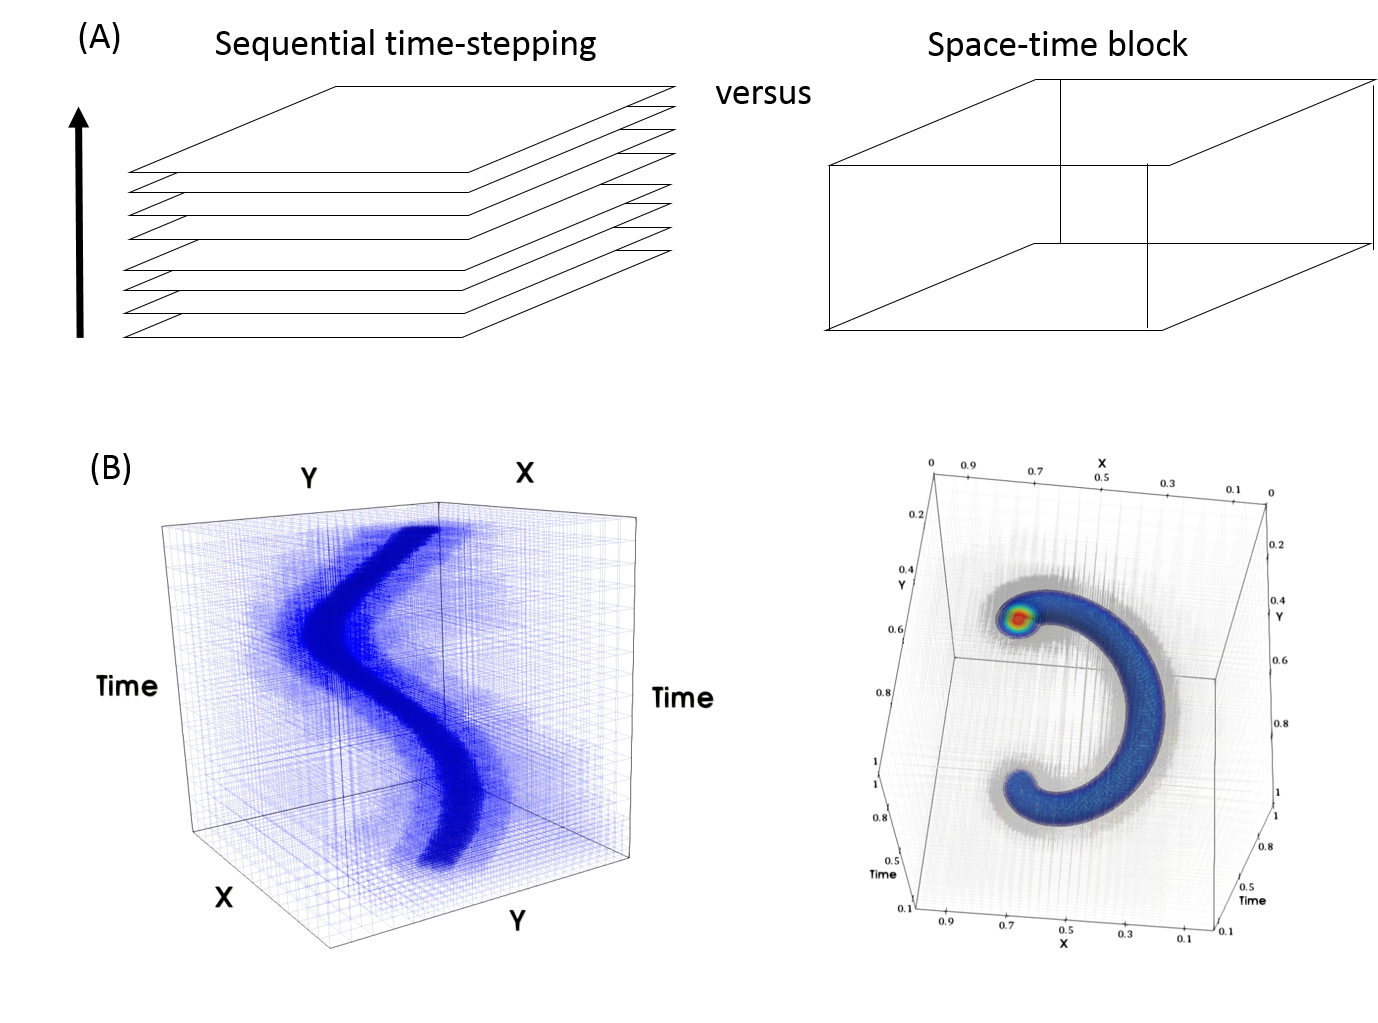
\includegraphics[width=0.48\textwidth]{figs/Picture2.png}
  %\begin{minipage}{15em}
  %\end{minipage}
  %\begin{minipage}[t]{0.5\textwidth}
  \caption{\label{fig:Overview} {\small (A) Conventional approaches to computationally solving evolution equations rely on marching sequentially in time. This limits parallel scalability to the spatial domain. In contrast, we present an approach for simultaneously solving for large blocks of spacetime. This approach not only exhibits good scalability, but also provides improved temporal convergence (proved via {\it a priori} estimates) as well as localized refinement in space and time based on  {\it a posteriori} error estimates. (B) Illustrative results in $2D~\texttt{space} + 1D ~\texttt{time}$ dimensions (i.e. 3D spacetime) for a rotating heat source problem. Notice that the mesh is refined in {\bf spacetime} only in regions of interest. This not only guarantees accurate solutions in space {\bf and} time, but is also substantially more efficient than the strategy of taking very small time steps  necessary to guarantee temporal accuracy in the sequential approach.}}
  %\end{minipage}
\end{figure}
% intro goes here. 

We present a $kD$ tree-based parallel strategy for solving with a {\it spacetime}-adaptive approach a general class of partial differential equations. This approach is primarily motivated by the necessity of designing computational methodologies that leverage the availability of very large computing clusters (exascale and beyond). For evolution problems, the standard approach of decomposing the spatial domain is a powerful paradigm of parallelization. However, for a fixed spatial discretization, the efficiency of purely spatial domain decomposition degrades substantially beyond a threshold -- usually tens of thousands of processors -- which makes this approach unsuitable on next generation machines. To overcome this barrier, a natural approach is to consider the time domain as an additional dimension and simultaneously solve for blocks of time, instead of the standard approach of sequential time-stepping. 

% \begin{figure*}[t]
%   \centering
%   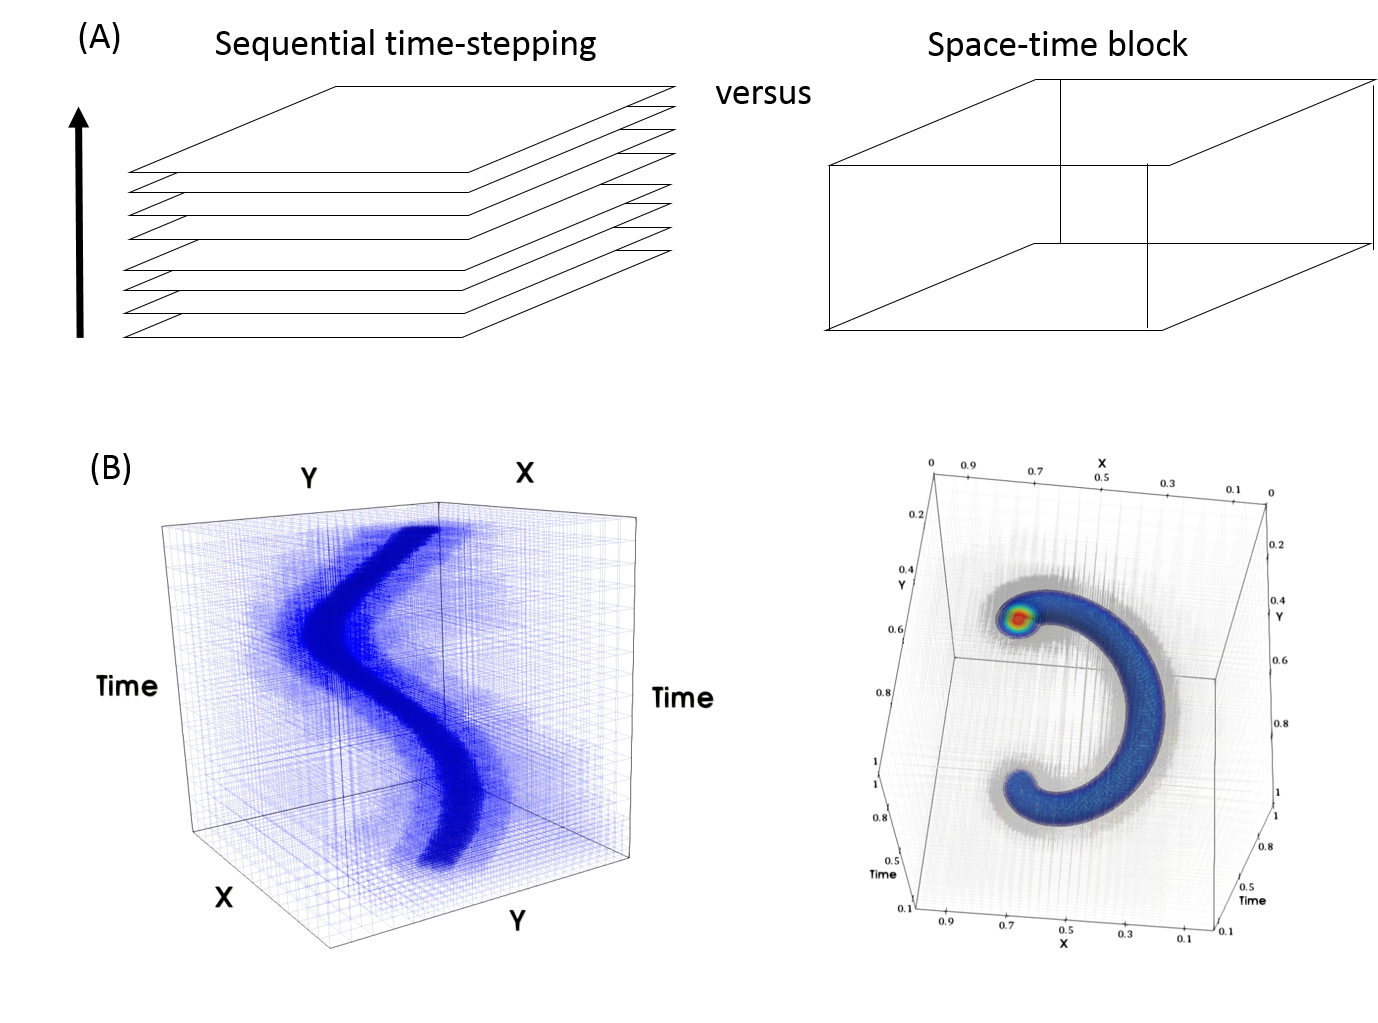
\includegraphics[width=0.7\textwidth]{figs/Picture2.png} \vspace{-0.35in}
%   \caption{\label{fig:Overview} {\small (A) Paradigm changing proposed work: Conventional approaches to computationally solving evolution equations rely on marching sequentially in time. This limits parallel scalability to the spatial domain. In contrast, we propose a paradigm breaking strategy of simultaneously solving for large blocks of spacetime. This will not only leverage next generation architectures, but will allow localized refinement in spacetime which will greatly streamline solution of a wide variety of evolution equations involving fronts and shocks. This opens up rich computational approaches for leveraging SPX: {\it a posteriori} error estimates, adjoints, preconditioner and solver designs as well as basic data structure design for solving problems in 4D space. (B) Preliminary results in $2D~\texttt{space} + 1D ~\texttt{time}$ dimensions (i.e. 3D spacetime) for a rotating heat source problem. Notice that the mesh is refined in {\bf spacetime} only in regions of interest. This not only guarantees accurate solutions in space {\bf and} time, but is also substantially more efficient than the strategy of taking very small time steps  necessary to guarantee temporal accuracy in the sequential approach.}} \vspace{-0.1in}
% \end{figure*}

This approach of solving for large blocks of spacetime is one of several promising approaches to time-parallel integration approaches that have been developed over the past century, but which are gaining increasing attention due to the availability of appropriate computing resources~\cite{50Years}. Broadly one can consider three types of parallelization approaches to solving a space-time problem. The first type of methods explicitly parallelizes only over time, and leaves spatial parallelism (and spatial adaptivity) undefined~\cite{parareal2001,falgout2014parallel}. These methods may also be considered as shooting methods~\cite{50Years}. The second type of methods explicitly parallelizes over space, and leaves temporal parallelism (and temporal adaptivity) undefined. These methods include wave form relaxation methods that attempt to reconcile the solution at spatial boundaries between space-time blocks~\cite{50Years}. The third type of methods explicitly targets parallelism (and adaptivity) in space and time. The current work seeks to advance type three methods. In the more narrow context of finite element methods, early work on type three methods was considered by Hughes and coworkers~\cite{hughes1996space,hughes1988space}, Tezduyar et al.~\cite{tezduyar2006space}, and Potanza and Reddy~\cite{pontaza2003spectral}, while variations on this theme have recently been explored by several groups~\cite{behr2008simplex, carey2010blockwise, lowrie1998space, mani2011efficient, rendall2012conservative, wang2015high}. 

%This approach of solving for large blocks of spacetime is one of several promising approaches to time parallel integration approaches that have been developed over the past century, but which are gaining increasing attention due to the availability of appropriate computing resources~\cite{50Years}. These include (a) shooting type time parallel methods that recursively improve 'initial' conditions at each time block ~\cite{parareal2001}, (b) wave form relaxation methods that attempt to reconcile solution at spatial boundaries between space time blocks, and (c) direct solutions in spacetime, where the complete spacetime block is discretized and reformulated into boundary value problems. 

Our preliminary work~\cite{dyja2018parallel} using the Finite Element Method (FEM) indicates that the third approach is particularly promising (see Fig.~\ref{fig:Overview}) as it provides a natural way to integrate mathematical analysis including construction of finite element error estimates (both {\it a priori} as well as {\it a posteriori}), and numerical stabilization of FEM solutions to advection-dominated equations, with foundation developments in scalable, parallel algorithms. The finite element method (FEM) is a widely popular numerical approach to solving partial differential equations, with multiple billions/year spent in CAD and CAM (computer aided design and manufacturing) based FEM software alone~\cite{Hughes_iso_book}. Its popularity arises from a compelling set of properties including (a) the ability to model arbitrary geometries, (b) the ability to seamlessly change order of representation (linear, quadratic and higher order), (c) the ability to utilize variational arguments that guarantee monotonic convergence to the solution with improved discretization, and (d) the ability to seamlessly utilize {\it a posteriori} error estimates to adapt the mesh. 

Solving for blocks of space-time provides a natural approach for effective usage of exascale computing resources~\cite{siam2013}, as well as leveraging novel architectures that exhibit extreme parallelism and deep memory hierarchies. In addition to this obvious advantage, this strategy provides the following advantages:
\begin{itemize}%[label={},nosep,leftmargin=1em,labelwidth=*,align=left]%\vspace{-0.15in}
    %\setlength\itemsep{0em}
    \item Solving for spacetime blocks also allows natural incorporation of {\it a posteriori} error estimates for spacetime mesh adaptivity. This has several additional tangible benefits in the context of computational overhead. For evolution problems -- including wave equations, and problems involving moving interfaces like bubbles and shocks -- that exhibit \text{``localized''} behavior in space and time, solving in blocks of spacetime that are locally refined to match the local behavior provides substantial computational gain~\cite{carey_estep}. An illustration (in lower dimensions) of this advantage (in $2D~\texttt{space} + 1D ~\texttt{time}$) is shown in Fig.~\ref{fig:Overview}(B), where the refined mesh is localized along the regions of high gradient of the solution.
    \item Solving in spacetime provides easy access to the full time history of the solution which is essential for the solution of design/inverse problems involving adjoints~\cite{Baskar1,Baskar2}
    \item Solving PDE's in spacetime removes any time-stepping constraints (like the CFL condition) on the numerical approach as the solution across all time-steps are simultaneously solved. This concept is illustrated in Fig.~\ref{fig:Overview}(B). The temporal discretization far away from the oscillating source is $2^5$ times larger than the smallest temporal discretization. This large variation in time step has no impact on numerical stability, which is an advantage over conventional sequential time stepping approaches.
    \item Finally, considering time as an additional dimension allows us to harness the benefits of using higher order basis functions to get high order accurate temporal schemes for no additional implementation cost (since these basis functions are already available for the spatial discretization). We derive theoretical {\it a priori} estimates of convergence with basis order and mesh size, and show that temporal error scales as a power of the mesh size in space time $|u - u_e|_2 \leq Ch^{\alpha}$, where $\alpha = \texttt{order of basis function} + 1$. Fig.~\ref{fig:ST_conv} computationally illustrates this point. We solve a 2D transient problem in spacetime on a 3D mesh. Using cubic basis functions is equivalent to a multi-step fourth order Runge-Kutta scheme for the sequential time stepping problem. 
\end{itemize}

\begin{figure}%{r}{0.5\textwidth}
\vspace{-0.2in}
  \begin{center}
 % \hspace{-3in}
    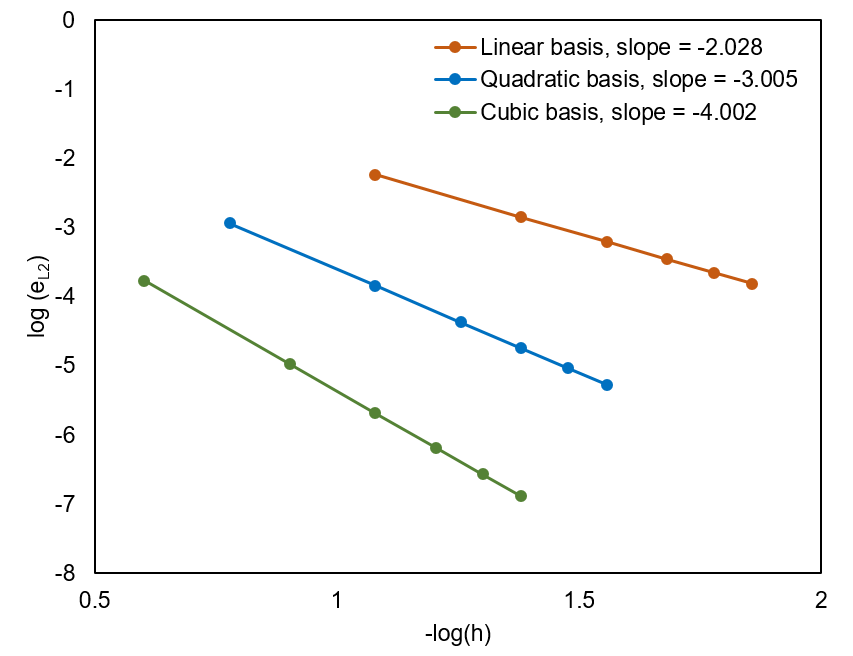
\includegraphics[trim={0 0 0 0},clip,width=0.48\textwidth]{figs/cnv-NL-final-time}
  \end{center}
   \vspace{-0.1in}
   \caption{\label{fig:ST_conv} \small Considering time to be another dimension allows easy use of higher order basis functions to get high order temporal accuracy. The figure illustrates how switching from linear to quadratic to cubic basis functions (for the problem solved in  Fig.~\ref{fig:Overview}B) in spacetime is equivalent to multi-step Runge Kutta methods of order 2, 3 and 4, respectively. }
   \vspace{-0.1in}
\end{figure}

\par Additionally, we break mesh-based abstractions for performing finite element (FEM) computations on adaptive spacetime meshes with the objective of achieving high performance and scalability on current and future architectures with extreme levels of parallelism and deep memory hierarchies. The new abstractions are designed to support matrix-free abstractions since these are important for large-scale parallelism. In addition, the new abstractions will enable code portability, for both CPU and GPU architectures. 

Our contributions in this paper are as follows: 
(a) we develop efficient $4D$ adaptive mesh construction and 2:1 balancing algorithms, 
(b) we develop a mesh-free matrix-free algorithms for finite element computations using a spacetime formulation, 
(c)  we derive both {\it a priori} error estimates, as well as residual based {\it a posteriori} error estimates for a canonical problem -- the linear time dependent heat diffusion equation, and numerically illustrate the theoretically determined improved convergence behavior of the space-time solution approach, and 
(d) we compare the scaling behavior of sequential time stepping method with the space-time approach. %the Crank Nicholson time - stepping method with the coupled space - time formulation for the linear diffusion equation with linear basis function.  

%Additionally, we formulate the \textit{aposteriori} error estimate for the coupled space - time formulation for the diffusion equations.  


%Our goal is to evaluate using x64, Intel Xeon Phi, Power8/9 and nVidia GPUs. In addition, since several linear solvers - such as geometric multigrid - depend on mesh information, we will develop solver realizations for our mesh-free abstractions.

%Finally, the outcome of this abstraction breaking approach to rethink FEM simulations of partial differential equations will be illustrated using two very impactful application examples in (a) flow and charge transport in complex heterogeneous porous films (energy harvesting)~\cite{kodali2012computer,kodali2012computational,wodo2015automated}, and (b) rapid evaluation of contaminant dispersal in urban neighborhoods~\cite{fontanini2017contaminant,fontanini2016methodology} (infrastructure and safety). This integration of a paradigm shifting approach to scientific computing with targeted, societally impactful applications is driven by the NSF mandate on Convergence thinking.



\section{Background: Space-time setting and error estimates}
\label{sec:background}
% background goes here. 

We present here a brief mathematical formulation of our canonical problem - the time dependent linear heat diffusion equation - in the space-time setting. We define our spatial domain as $U \in \mathbb{R}^n$, where $U$ is an open and bounded domain, with $n = 1, 2, \text{or} 3$. We consider the time horizon $I_{_T} = (0,T\in \mathbb{R^+})$ is a bounded time interval. Then we define the space-time domain as the Cartesian product of these two domains, $\Omega = U \times I_{_T} = U\times(0,T)$. Denote the overall boundary of this space-time domain as $\Gamma = \partial \Omega$. In particular, the spatial domain boundary is defined as $\Gamma_{_U} = \partial U \times (0,T)$ and the time boundaries are defined as $\Gamma_{_0} = U\times\{0\}$ and $\Gamma_{_T} = U\times\{T\}$ which are the initial and final time boundaries respectively. Note that $\Gamma = \Gamma_{_U}\cup\Gamma_{_0}\cup\Gamma_{_T}$. Finally we also define the closure of $\Omega$ as $\bar{\Omega} = \Omega \cup \Gamma$

The canonical equation we are interested is the following equation for the scalar space-time field $u: \Omega \rightarrow \mathbb{R}$:
\begin{subequations}\label{eq:linearheat}
\begin{align}
    \partial_t u - \nabla\cdot(\kappa\nabla u) &=f \quad \textrm{in}\quad\Omega\\
u&=0\quad \textrm{on}\quad\Gamma_U\\
u(\cdot,t_0)&=u_0\quad \textrm{on}\quad \Gamma_{0}
\end{align}
\end{subequations}
where $f: \Omega \rightarrow \mathbb{R}$ is a smooth forcing function, $\kappa > 0$ has no dependence on $u$, and $\nabla$ denotes the spatial gradient operator. We assume that Dirichlet conditions are imposed on the boundary $\Gamma_U$. 
%Also, $\nabla$ denotes the spatial gradient operator in $\mathbb{R}^n$, e.g., for $n=3$ we have,
%\begin{equation}
%    \nabla = \frac{\partial}{\partial x} +
%    \frac{\partial}{\partial y} +
%    \frac{\partial}{\partial z}
%\end{equation}

Next we define suitable function spaces for the trial and test functions used in the variational formulation. We define the space of the trial functions as $V_u = \left\{u\in H^1(\Omega): u|_{\Gamma_{_U}} = 0, u|_{_{\Gamma_0}} = u_0 \right\}$ and the space of the test functions as $V_v = \left\{v\in H^1(\Omega): v|_{\Gamma_{_U}\cup\Gamma_0} = 0\right\}$. The continuous variational problem problem is posed as follows: find $u\in V_u$ such that,
\begin{equation}\label{eq:continuous-variational-form}
    a(u, v) = l(v)\quad \forall v \in V_v
\end{equation}
where,
\begin{align}\label{def:continuous-bilinear-form}
    a(u,v) &= (\partial_t u, v) + (\kappa \nabla u, \nabla v)\\
    l(v) &= (f,v)
\end{align}
Here $(\cdot,\cdot)$ denotes the usual inner product in $L^2(\Omega)$. Note that the inner product is over the space-time domain, $(a,b) = \int_0^T \int_U a.b dx dt$. The finite dimensional approximation of these spaces are denoted as $V^h_u$ and $V^h_v$, and 
\begin{multline}
    V^h_u := \{u^h \mid u^h \in H^1(\Omega), \quad u^h\in P(\Omega ^K) \quad \forall K,\\
    \quad u^h|_{\Gamma_{_U}} = 0 \qquad\textrm{and}\quad u^h|_{\Gamma_{0}} = u_{0}\}
\end{multline}
\begin{align}
    V^h_v := \{v^h \mid v^h \in H^1(\Omega), \quad v^h\in P(\Omega^K) \quad \forall K, \quad v^h|_{\Gamma_{_0}\cup\Gamma_{_U}} = 0\}
\end{align}
where $P(\Omega ^K)$ being the space of the standard polynomial finite element shape functions on element $\Omega^K$. 

Numerical solutions to Equation~\ref{eq:linearheat} can exhibit numerical instabilities because the bilinear form $a(u,v)$ in Equation~\ref{eq:continuous-variational-form} is not strongly coercive in $V_u$. Therefore, following~\cite{langer2016space}, we add a correction term to the bilinear form making the the modified bilinear form stable. The discrete variational problem along with this stabilization is given by,
\begin{equation}\label{eq:discrete-variational-form}
    a(u^h, v^h) = l(v^h)\quad \forall v \in V_v
\end{equation}
\begin{multline}\label{def:discrete-bilinear-form}
    a^h(u^h,v^h) = (\partial_t u^h, v^h) + \delta (\partial_t u^h, \partial_t v^h) + (\kappa \nabla u, \nabla v) \\
     + \delta (\nabla u^h,\nabla \partial_t v^h)
\end{multline}
\begin{align}\label{def:discrete-linear-form}
    l^h(v^h) &= (f,v^h) + \delta(f,\partial_t v^h)
\end{align}
for all $v^h \in V^h_v$. $\delta$ is a mesh dependent parameter proportional to the mesh size $h$.

This discrete bilinear form is bounded and also coercive on $V^h_v$ with respect to the norm
\begin{align}
    \|u^h\|_{V_{u}} = \left[ \nabla u^h\|^2_{L^2(\Omega)} + \delta\|\partial_t u^h\|^2_{L^2(\Omega)} + \frac{1}{2}\|u^h\|^2_{L^2(\Gamma_{_T})} \right]
\end{align}
Since the linear form given by Equation~\ref{def:discrete-linear-form} is also bounded, the generalized Lax-Milgram Lemma guarantees a unique solution. 

Denoting the solution to Equation~\ref{eq:continuous-variational-form} by $u$ and the solution to Equation~\ref{eq:discrete-variational-form} by $u^h$, we derive the \textit{a priori} error estimate as
\begin{align}\label{estimate:a-priori}
    \|u - u^h\|_{V^h_u} \leq Ch^{p+1}\|u\|_{H^{p+1}(\Omega)}
\end{align}
where $p$ is the highest degree of the polynomial space to which $u^h$ belongs, $h$ is the size of the space-time element, and some constant $C$. Note that this estimate guarantees high order temporal accuracy (essentially, equivalent to a $p+1$-th order time stepper) when using a $p^{th}$ order basis function. We numerically illustrate this powerful result in Fig.~\ref{fig:ST_conv}, where we solve a problem with a rotating heat source with an analytically known solution. We plot the $L_2$ error (over the space-time domain) between the analytical solution and the computed solution using different order of basis functions. The mesh convergence plots clearly illustrate the expected change in slope from linear to quadratic to cubic basis functions. This is equivalent to a sequential time stepper, specifically a multi-step Runge Kutta methods of order 2, 3 and 4, respectively.

%[BG] Why is this statement needed? Note that, in all the numerical examples in this paper, the forcing function $f\in C^{\infty}(\Omega)$ , therefore $u\in C^{\infty}(\Omega)$ for the continuous problem.

Finally, based on the calculated solution $u^h$, we can formulate an \textit{a posteriori} error estimate. We use the residual based approach~\cite{ainsworth_oden, verfurth2013} that associates an error estimate with each space-time element in the 4D tree. This error estimate will inform adaptive space-time refinement of the domain. The residual based \textit{a posteriori} error estimator for a space-time element $K$ is given by:
\begin{align}
    \eta_{_K}=\left\{h_K^2 \left\| \bar{f}_K+\nabla\cdot\kappa\nabla u_h - {\partial_t u_h}\right\|_K^2+\frac{1}{2}\sum_{E\in\mathcal{E}_{K}}h_E\left\|\mathbb{J}_E(\mathbf{n}_E\cdot\nabla u_h)\right\|_E^2\right\}^\frac{1}{2}
\end{align}
where $\mathcal{E}$ denotes the set of all edges of element $K$, $\mathbb{J}$ denotes the jump in the gradient of the solution $u^h$ across those edges and $\bar{f}_K$ denotes the average force value in the element $K$. This \textit{a posteriori} error is calculated elementwise and a suitable refinement strategy is adopted (see next section) for space-time mesh refinement. 

We emphasize that while the conceptual formulation of a PDE solution strategy in space-time blocks is not new, the rigorous formulation of both {\it a priori} and {\it a posteriori} error estimates is a novel contribution. In particular, the {\it a priori} error estimates provide theoretical guarantees of enhanced convergence which serve as rigorous tests of our numerical implementation.

%\hs{Please review this paragraph}
In what follows, the finite element mesh is generated through a $kD$-tree based locally regular octant (for 3D) or \stra~(for 4D) objects (leaves in the $kD$-tree as explained later). This mesh is
not explicitly saved as explained in the next section, and the mesh information is deduced on-the-fly. This is a very efficient way of implementing the continuous Galerkin method through a locally structured mesh. Each of the leaves in the $kD$-tree embodies a finite element which can then be projected onto a isoparametric space through an affine transformation. All calculations for the domain integration are performed in this isoparametric space and then transformed back to the physical space.  


\section{Methodology}
\label{sec:methodology}
% methods goes here. 
In this section, we present our \textit{comparison-free},\textit{matrix-free}, \textit{mesh-free} algorithms for performing FEM computations on $kD$ trees. Several state-of-the-art approaches \cite{FernandoDendroGR, Dendro, SundarSampathBiros08, SundarMalhotraBiros13, dealII90, mfem} use a comparison operator induced by a Space Filling Curve (SFC) to sort and partition the nodes of the tree\cite{FernandoSundar16}. The matrix-free FEM computations are widely used in the HPC community\cite{Dendro, mantle, dealII90, mfem}, due to better scalability compared to the matrix-based approaches. Here matrix-free FEM approaches refer to FEM computations without the explicit assembly of matrices,  instead providing a matrix-vector product (\mvec). These are also particularly efficient for non-linear operators, which would require repeated assembly. 
%
For performing matrix assembly or a \mvec\, we need neighborhood data structures such as \textit{element to nodal mapping} or \textit{nodal to nodal mapping}. 
We refer to such data structures % used to perform numerical computations,we refer to
as the mesh (connectivity information).

There are several major drawbacks of comparison- and mesh- based numerical computations on adaptive trees. 
Firstly, since the elements are ordered based on the SFC, it is possible to use binary search to find neighbors among the list of elements. However, for large numbers of elements (as in the case of $4D$), this can result in memory access forcing a cache misses least for the initial few accesses. Secondly, despite the locality of the SFC, neighbors are not contiguous in memory. During an assembly/\mvec\ operation, the separation between neighbours will cause inefficient memory access. More importantly, the use of a mesh causes indirect memory access of the variable (\mintinline{C++}{u[mesh[elem,node]]} instead of \mintinline{C++}{u[node++]}), making it difficult for compilers to prefetch data. 
% The  ordering of the tree leaf nodes is used to perform, binary search operations in order to build the above neighborhood data structures. The binary search operations result in unstructured memory accesses leading to bad memory performances especially the number of search keys increases (see Figure \ref{}). 
%
% The mesh-based FEM computations require indirect memory accesses to the underlying variables defined on the grid \mf{if disable the ability to prefetch the data, in streaming processor architectures} (see Figure). 
%
As the dimensionality $k$ increases, building neighborhood data structures becomes extremely complex, increases storage, and makes the algorithm computationally expensive. The last factor is particularly important for problems requiring frequent mesh-refinements. 

In order to overcome the above challenges we propose a mesh-free \mvec\ that avoids these issues by computing the neighborhood information on the fly, similar to how matrix-free methods work without explicitly storing the matrix entries. We therefore end up with a 
%
\textit{comparison-free, mesh-free, matrix-free} algorithm for performing FEM computations on $kD$ trees. 

\subsection{\tsort: comparison-free SFC based tree partitioning}
\label{subsec:tsort}
Given that we are interested in generating a space-traversal, more so of application specific coordinates or regions, it is efficient to consider this problem as a traversal of the points in the SFC order. Specifically, we construct the tree in a \textit{top-down} fashion, one level at a time, arranging the nodes at a given level based on the recurrence rules for the specific SFC. We call this algorithm \tsort ~(Algorithm~\ref{alg:tsort}). There are two main advantages for this approach: 1). The comparison-free property makes the structure of \tsort~ independent of the SFC being used\cite{FernandoDuplyakinSundar17}. 2). The top-down traversal of the tree in breadth-first fashion, which is performed in the distributed \tsort~, gives us explicit control over the  load-imbalance, which can be tuned as specified in \cite{FernandoSundar16}. All subsequent operations, such as tree construction, enforcing 2:1 balancing, and the \mvec~ operation in FEM computations, are performed using top-down and bottom-up traversals with slight variations of the sequential \tsort~ algorithm. 

\begin{algorithm}[t]
  \caption{\tsort}\label{alg:tsort}
  \footnotesize
  \begin{algorithmic}[1]
    \Require A list of points or regions $W$, the starting level $l_1$ and the ending level $l_2$
    \Ensure $W$ is reordered according to the SFC.
    %\Function{TreeSort($W$, $l_1$, $l_2$)}{}
    \State $counts [] \leftarrow 0$
    \Comment $|counts| = 2^{d}$, 16 for $4D$
    \For{$w \in W$}
    \State increment $counts[child\_num(w)]$
    \EndFor
    % Bucket($W$, $l$) 
    \State $counts [] \leftarrow R_h(counts)$ 
    \Comment Permute counts using SFC ordering
    \State offsets [] $\leftarrow scan(counts)$
    \For{$w \in W$}
    \State $i\leftarrow child\_num(w)$
    \State append $w$ to $W_i$ at offsets$[i]$
    \State increment offset$[i]$
    \EndFor 
    \If{$l_1 > l_2$} 
    \For{$i:=1:2^{d}$}
    \State \tsort ($W_i, l_1-1, l_2$)
    \Comment local sort
    \EndFor 
    \EndIf
    %\EndFunction
    \State \Return $W$
  \end{algorithmic}
\end{algorithm}

\begin{algorithm}[t]
  \caption{\dsort: Distributed \tsort}\label{alg:dsort}
  \footnotesize
  \begin{algorithmic}[1]
    \Require A distributed list of points or regions $W_r$, $\mathit{comm}$, $p$ (w.l.g., assume $p= mk$),
    $p_r$ of current task in $\mathit{comm}$, $tol$ load flexibility, 
    \Ensure globally sorted array $W$
    %\State $split\_count \leftarrow 1$
    \State $counts\_local \leftarrow [\ ], counts\_global \leftarrow [\ ]$    
    \State $s [] \leftarrow \tsort(W_r,l-\log(p),l)$ \Comment initial splitter computation
    
    \While {$|s_r-\frac{rn}{p}|>tol$}     
    \State $counts[] \leftarrow 0$ \Comment $|counts| = 2^{d}$, 16 for 4D
    \For{$w \in W$}
    \State increment $counts[child\_num(w)]$
    \EndFor
    \State $counts\_local [] \leftarrow push(counts)$  
    \State $counts [] \leftarrow R_h(counts)$ 
    \Comment Permute counts using SFC ordering
    \State offsets $[] \leftarrow scan(counts)$
    \For{$w \in W$}
    \State $i\leftarrow child\_num(w)$
    \State append $w$ to $W_i$ at offsets$[i]$
    \State increment offset$[i]$
    \EndFor
    %\State $split\_count \leftarrow 2^{dim}\times split\_count$

    \State $\mathtt{MPI\_ReduceAll}(counts\_local,counts\_global,comm)$
    \State $s[] \leftarrow select(s,counts\_global)$
    \EndWhile
    %	  \State $\mathtt{MPI\_AlltoAllv}$(A,splitters,comm)
    % \Comment optimal splitter computation (with in the given tolerance)	  
    \State $\mathtt{MPI\_AlltoAllv}$(A,splitters,comm)
    \Comment Staged All2all
    \State \tsort$(W_r, 0, l)$ \Comment local sort
    \State \Return $W_r$
  \end{algorithmic}
\end{algorithm}


\begin{figure}
	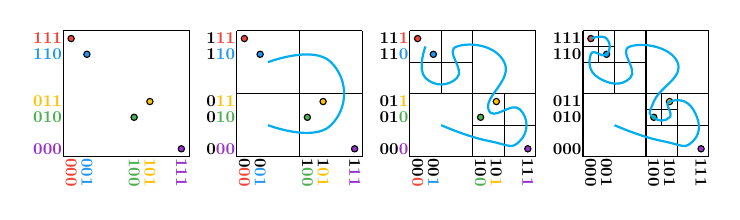
\begin{tikzpicture}[scale=0.2,every node/.style={scale=0.6}]
	% \draw[gray, very thin] (0,0) grid +(8,8);
	\draw (0,0) rectangle +(8,8);
	\draw[fill=cpu3] (0.5,7.5) circle (0.2);
	\draw[fill=cpu4] (1.5,6.5) circle (0.2);
	\draw[fill=cpu1] (4.5,2.5) circle (0.2);
	\draw[fill=cpu2] (5.5,3.5) circle (0.2);
	\draw[fill=cpu5] (7.5,0.5) circle (0.2);
	
	\begin{scope}[shift={(11,0)}]
	\draw[step=4] (0,0) grid +(8,8);
	\draw[fill=cpu3] (0.5,7.5) circle (0.2);
	\draw[fill=cpu4] (1.5,6.5) circle (0.2);
	\draw[fill=cpu1] (4.5,2.5) circle (0.2);
	\draw[fill=cpu2] (5.5,3.5) circle (0.2);
	\draw[fill=cpu5] (7.5,0.5) circle (0.2);

	\draw [cyan,thick, xshift=0cm] plot [smooth, tension=1] coordinates { (2,2) (6,2) (6,6) (2,6)};
	
	\node at (-1,7.5) {$\mathbf{1}$\textcolor{cpu3}{$\mathbf{1 1}$}};
	\node at (-1,6.5) {$\mathbf{1}$\textcolor{cpu4}{$\mathbf{1 0}$}};
	\node at (-1,3.5) {$\mathbf{0}$\textcolor{cpu2}{$\mathbf{1 1}$}};
	\node at (-1,2.5) {$\mathbf{0}$\textcolor{cpu1}{$\mathbf{1 0}$}};
	\node at (-1,0.5) {$\mathbf{0}$\textcolor{cpu5}{$\mathbf{0 0}$}};
	
	\node[rotate=-90] at (0.5,-1) {$\mathbf{0}$\textcolor{cpu3}{$\mathbf{0 0}$}};
	\node[rotate=-90] at (1.5,-1) {$\mathbf{0}$\textcolor{cpu4}{$\mathbf{0 1}$}};
	\node[rotate=-90] at (5.5,-1) {$\mathbf{1}$\textcolor{cpu2}{$\mathbf{0 1}$}};
	\node[rotate=-90] at (4.5,-1) {$\mathbf{1}$\textcolor{cpu1}{$\mathbf{0 0}$}};
	\node[rotate=-90] at (7.5,-1) {$\mathbf{1}$\textcolor{cpu5}{$\mathbf{1 1}$}};
	\end{scope}
	
	\begin{scope}[shift={(22,0)}]
	\draw[step=4] (0,0) grid +(8,8);
	\draw[step=2] (4,0) grid +(4,4);
	\draw[step=2] (0,4) grid +(4,4);
	\draw[fill=cpu3] (0.5,7.5) circle (0.2);
	\draw[fill=cpu4] (1.5,6.5) circle (0.2);
	\draw[fill=cpu1] (4.5,2.5) circle (0.2);
	\draw[fill=cpu2] (5.5,3.5) circle (0.2);
	\draw[fill=cpu5] (7.5,0.5) circle (0.2);
	
	\node at (-1,7.5) {$\mathbf{11}$\textcolor{cpu3}{$\mathbf{1}$}};
	\node at (-1,6.5) {$\mathbf{11}$\textcolor{cpu4}{$\mathbf{0}$}};
	\node at (-1,3.5) {$\mathbf{01}$\textcolor{cpu2}{$\mathbf{1}$}};
	\node at (-1,2.5) {$\mathbf{01}$\textcolor{cpu1}{$\mathbf{0}$}};
	\node at (-1,0.5) {$\mathbf{00}$\textcolor{cpu5}{$\mathbf{0}$}};
	
	\node[rotate=-90] at (0.5,-1) {$\mathbf{00}$\textcolor{cpu3}{$\mathbf{0}$}};
	\node[rotate=-90] at (1.5,-1) {$\mathbf{00}$\textcolor{cpu4}{$\mathbf{1}$}};
	\node[rotate=-90] at (5.5,-1) {$\mathbf{10}$\textcolor{cpu2}{$\mathbf{1}$}};
	\node[rotate=-90] at (4.5,-1) {$\mathbf{10}$\textcolor{cpu1}{$\mathbf{0}$}};
	\node[rotate=-90] at (7.5,-1) {$\mathbf{11}$\textcolor{cpu5}{$\mathbf{1}$}};
	\draw [cyan,thick, xshift=0cm] plot [smooth, tension=1] coordinates { (2,2) (5,1) (7,1) (7,3) (5,3) (6,6) (3,7) (3,5) (1,5) (1,7)};
	\end{scope}
	
	\begin{scope}[shift={(33,0)}]
	\draw[step=4] (0,0) grid +(8,8);
	\draw[step=2] (4,0) grid +(4,4);
	\draw[step=2] (0,4) grid +(4,4);
	\draw (0,6) grid +(2,2);
	\draw (4,2) grid +(2,2);
	
	\draw[fill=cpu3] (0.5,7.5) circle (0.2);
	\draw[fill=cpu4] (1.5,6.5) circle (0.2);
	\draw[fill=cpu1] (4.5,2.5) circle (0.2);
	\draw[fill=cpu2] (5.5,3.5) circle (0.2);
	\draw[fill=cpu5] (7.5,0.5) circle (0.2);
	
	\node at (-1,7.5) {$\mathbf{111}$};
	\node at (-1,6.5) {$\mathbf{110}$};
	\node at (-1,3.5) {$\mathbf{011}$};
	\node at (-1,2.5) {$\mathbf{010}$};
	\node at (-1,0.5) {$\mathbf{000}$};
	
	\node[rotate=-90] at (0.5,-1) {$\mathbf{000}$};
	\node[rotate=-90] at (1.5,-1) {$\mathbf{001}$};
	\node[rotate=-90] at (5.5,-1) {$\mathbf{101}$};
	\node[rotate=-90] at (4.5,-1) {$\mathbf{100}$};
	\node[rotate=-90] at (7.5,-1) {$\mathbf{111}$};
	\draw [cyan,thick, xshift=0cm] plot [smooth, tension=1] coordinates { (2,2) (5,1) (7,1) (7,3) (5.5,3.5) (5.5,2.5) (4.5,2.5) (4.5,3.5) (6,6) (3,7) (3,5) (1,5) (0.5,6.5) (1.5,6.5) (1.5,7.5) (0.5,7.5)};
	\end{scope}
	
	\node at (-1,7.5) {\textcolor{cpu3}{$\mathbf{1 1 1}$}};
	\node at (-1,6.5) {\textcolor{cpu4}{$\mathbf{1 1 0}$}};
	\node at (-1,3.5) {\textcolor{cpu2}{$\mathbf{0 1 1}$}};
	\node at (-1,2.5) {\textcolor{cpu1}{$\mathbf{0 1 0}$}};
	\node at (-1,0.5) {\textcolor{cpu5}{$\mathbf{0 0 0}$}};

	\node[rotate=-90] at (0.5,-1) {\textcolor{cpu3}{$\mathbf{0 0 0}$}};
	\node[rotate=-90] at (1.5,-1) {\textcolor{cpu4}{$\mathbf{0 0 1}$}};
	\node[rotate=-90] at (5.5,-1) {\textcolor{cpu2}{$\mathbf{1 0 1}$}};
	\node[rotate=-90] at (4.5,-1) {\textcolor{cpu1}{$\mathbf{1 0 0}$}};
	\node[rotate=-90] at (7.5,-1) {\textcolor{cpu5}{$\mathbf{1 1 1}$}};
	
%	\node at (12,-1) {$\mathbf{0}$};
%	\node at (16,-1) {$\mathbf{1}$};
%	
%	\node at (9,2) {$\mathbf{0}$};
%	\node at (9,6) {$\mathbf{1}$};
	
	\end{tikzpicture}
	\caption{\label{fig:tsort} Bucketing each point and reordering the buckets based on the SFC ordering at each level $l$ with top-down traversal. Each color-coded point is represented by its $x$ and $y$ coordinates. From the MSD-Radix perspective, we start with the most-significant bit for both the $x$ and $y$ coordinates and progressively bucket (order) the points based on these. The bits are colored based on the points and turn black as they get used to (partially) order the points.}
\end{figure}

\subsection{Hilbert curve/ordering in $4D$}
\label{subsec:hilbert4d}
The comparison-free structure of \tsort~ allows us to use any SFC. In our work we are interested in the Hilbert curve.

The Hilbert curve is an SFC with the property that adjacent segments in the curve are mapped to adjacent regions in space. Previous works have exploited this property to better preserve spatial locality in linearized octrees, thus curbing the communication cost of partitioning a spatial domain \cite{FernandoSundar16}.

Extending the Hilbert curve to any dimension beyond 2D is nontrivial. Although a known three-dimensional extension was used previously \cite{FernandoSundar16}, certainly the situation is more complicated in four dimensions. Not only does it become tedious to write (and reason about) a permutation table of recurrence rules, but also the Hilbert curve does not have a unique high-dimensional extension. One must choose a definition among the many possible SFCs that satisfy the above locality property.

Haverkort \cite{haverkort2012harmonious} provides
\begin{itemize}
  \item an additional constraint (``interdimensional consistency'') that uniquely characterizes the so-called \textit{harmonious} Hilbert curve in any dimension;
  \item a systematic constructive definition for the curve in any dimension.
\end{itemize}

(The idea of interdimensional consistency is that the restriction of the curve to a face should be the same curve, but a lower-dimensional version. Potential benefits include hardware optimization and/or better locality \cite{haverkort2012harmonious}.)

Based on Haverkort's abstract recurrence rules, we can programmatically generate SFC rotation tables for the Hilbert curve in four dimensions, and higher. More detailed description is given in \ref{subsec:4d_hilbert}.

\subsection{$kD$-Tree Construction}
\label{subsec:tconst}

\begin{figure}
	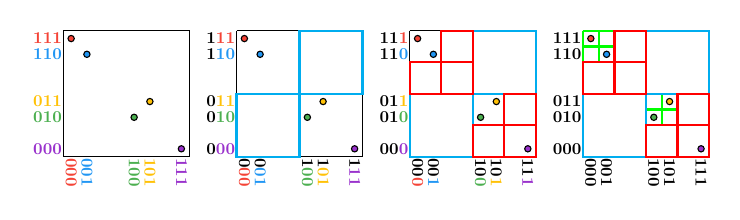
\begin{tikzpicture}[scale=0.2,every node/.style={scale=0.6}]
	% \draw[gray, very thin] (0,0) grid +(8,8);
	\draw (0,0) rectangle +(8,8);
	\draw[fill=cpu3] (0.5,7.5) circle (0.2);
	\draw[fill=cpu4] (1.5,6.5) circle (0.2);
	\draw[fill=cpu1] (4.5,2.5) circle (0.2);
	\draw[fill=cpu2] (5.5,3.5) circle (0.2);
	\draw[fill=cpu5] (7.5,0.5) circle (0.2);
	
	\begin{scope}[shift={(11,0)}]
	\draw[step=4] (0,0) grid +(8,8);
	\draw[cyan,thick] (0,0) rectangle +(4,4);
	\draw[cyan,thick] (4,4) rectangle +(4,4);
	\draw[fill=cpu3] (0.5,7.5) circle (0.2);
	\draw[fill=cpu4] (1.5,6.5) circle (0.2);
	\draw[fill=cpu1] (4.5,2.5) circle (0.2);
	\draw[fill=cpu2] (5.5,3.5) circle (0.2);
	\draw[fill=cpu5] (7.5,0.5) circle (0.2);
	
	\node at (-1,7.5) {$\mathbf{1}$\textcolor{cpu3}{$\mathbf{1 1}$}};
	\node at (-1,6.5) {$\mathbf{1}$\textcolor{cpu4}{$\mathbf{1 0}$}};
	\node at (-1,3.5) {$\mathbf{0}$\textcolor{cpu2}{$\mathbf{1 1}$}};
	\node at (-1,2.5) {$\mathbf{0}$\textcolor{cpu1}{$\mathbf{1 0}$}};
	\node at (-1,0.5) {$\mathbf{0}$\textcolor{cpu5}{$\mathbf{0 0}$}};
	
	\node[rotate=-90] at (0.5,-1) {$\mathbf{0}$\textcolor{cpu3}{$\mathbf{0 0}$}};
	\node[rotate=-90] at (1.5,-1) {$\mathbf{0}$\textcolor{cpu4}{$\mathbf{0 1}$}};
	\node[rotate=-90] at (5.5,-1) {$\mathbf{1}$\textcolor{cpu2}{$\mathbf{0 1}$}};
	\node[rotate=-90] at (4.5,-1) {$\mathbf{1}$\textcolor{cpu1}{$\mathbf{0 0}$}};
	\node[rotate=-90] at (7.5,-1) {$\mathbf{1}$\textcolor{cpu5}{$\mathbf{1 1}$}};
	\end{scope}
	
	\begin{scope}[shift={(22,0)}]
	\draw[step=4] (0,0) grid +(8,8);
	\draw[step=2] (4,0) grid +(4,4);
	\draw[step=2] (0,4) grid +(4,4);
	
	\draw[cyan,thick] (0,0) rectangle +(4,4);
	\draw[cyan,thick] (4,4) rectangle +(4,4);

	\draw[red,thick] (0,4) rectangle +(2,2);
	\draw[red,thick] (2,4) rectangle +(2,2);
	\draw[red,thick] (2,6) rectangle +(2,2);

	\draw[red,thick] (4,0) rectangle +(2,2);
	\draw[red,thick] (6,2) rectangle +(2,2);
	\draw[red,thick] (6,0) rectangle +(2,2);
	
	\draw[fill=cpu3] (0.5,7.5) circle (0.2);
	\draw[fill=cpu4] (1.5,6.5) circle (0.2);
	\draw[fill=cpu1] (4.5,2.5) circle (0.2);
	\draw[fill=cpu2] (5.5,3.5) circle (0.2);
	\draw[fill=cpu5] (7.5,0.5) circle (0.2);
	
	\node at (-1,7.5) {$\mathbf{11}$\textcolor{cpu3}{$\mathbf{1}$}};
	\node at (-1,6.5) {$\mathbf{11}$\textcolor{cpu4}{$\mathbf{0}$}};
	\node at (-1,3.5) {$\mathbf{01}$\textcolor{cpu2}{$\mathbf{1}$}};
	\node at (-1,2.5) {$\mathbf{01}$\textcolor{cpu1}{$\mathbf{0}$}};
	\node at (-1,0.5) {$\mathbf{00}$\textcolor{cpu5}{$\mathbf{0}$}};
	
	\node[rotate=-90] at (0.5,-1) {$\mathbf{00}$\textcolor{cpu3}{$\mathbf{0}$}};
	\node[rotate=-90] at (1.5,-1) {$\mathbf{00}$\textcolor{cpu4}{$\mathbf{1}$}};
	\node[rotate=-90] at (5.5,-1) {$\mathbf{10}$\textcolor{cpu2}{$\mathbf{1}$}};
	\node[rotate=-90] at (4.5,-1) {$\mathbf{10}$\textcolor{cpu1}{$\mathbf{0}$}};
	\node[rotate=-90] at (7.5,-1) {$\mathbf{11}$\textcolor{cpu5}{$\mathbf{1}$}};
	\end{scope}
	
	\begin{scope}[shift={(33,0)}]
	\draw[step=4] (0,0) grid +(8,8);
	\draw[step=2] (4,0) grid +(4,4);
	\draw[step=2] (0,4) grid +(4,4);
	\draw[green,thick] (0,6) grid +(2,2);
	\draw[green,thick] (4,2) grid +(2,2);
	
	\draw[cyan,thick] (0,0) rectangle +(4,4);
	\draw[cyan,thick] (4,4) rectangle +(4,4);

	\draw[red,thick] (0,4) rectangle +(2,2);
	\draw[red,thick] (2,4) rectangle +(2,2);
	\draw[red,thick] (2,6) rectangle +(2,2);

	\draw[red,thick] (4,0) rectangle +(2,2);
	\draw[red,thick] (6,2) rectangle +(2,2);
	\draw[red,thick] (6,0) rectangle +(2,2);	
	 	
	\draw[fill=cpu3] (0.5,7.5) circle (0.2);
	\draw[fill=cpu4] (1.5,6.5) circle (0.2);
	\draw[fill=cpu1] (4.5,2.5) circle (0.2);
	\draw[fill=cpu2] (5.5,3.5) circle (0.2);
	\draw[fill=cpu5] (7.5,0.5) circle (0.2);
	
	\node at (-1,7.5) {$\mathbf{111}$};
	\node at (-1,6.5) {$\mathbf{110}$};
	\node at (-1,3.5) {$\mathbf{011}$};
	\node at (-1,2.5) {$\mathbf{010}$};
	\node at (-1,0.5) {$\mathbf{000}$};
	
	\node[rotate=-90] at (0.5,-1) {$\mathbf{000}$};
	\node[rotate=-90] at (1.5,-1) {$\mathbf{001}$};
	\node[rotate=-90] at (5.5,-1) {$\mathbf{101}$};
	\node[rotate=-90] at (4.5,-1) {$\mathbf{100}$};
	\node[rotate=-90] at (7.5,-1) {$\mathbf{111}$};
	
	\end{scope}
	
	\node at (-1,7.5) {\textcolor{cpu3}{$\mathbf{1 1 1}$}};
	\node at (-1,6.5) {\textcolor{cpu4}{$\mathbf{1 1 0}$}};
	\node at (-1,3.5) {\textcolor{cpu2}{$\mathbf{0 1 1}$}};
	\node at (-1,2.5) {\textcolor{cpu1}{$\mathbf{0 1 0}$}};
	\node at (-1,0.5) {\textcolor{cpu5}{$\mathbf{0 0 0}$}};

	\node[rotate=-90] at (0.5,-1) {\textcolor{cpu3}{$\mathbf{0 0 0}$}};
	\node[rotate=-90] at (1.5,-1) {\textcolor{cpu4}{$\mathbf{0 0 1}$}};
	\node[rotate=-90] at (5.5,-1) {\textcolor{cpu2}{$\mathbf{1 0 1}$}};
	\node[rotate=-90] at (4.5,-1) {\textcolor{cpu1}{$\mathbf{1 0 0}$}};
	\node[rotate=-90] at (7.5,-1) {\textcolor{cpu5}{$\mathbf{1 1 1}$}};
	
%	\node at (12,-1) {$\mathbf{0}$};
%	\node at (16,-1) {$\mathbf{1}$};
%	
%	\node at (9,2) {$\mathbf{0}$};
%	\node at (9,6) {$\mathbf{1}$};
	
	\end{tikzpicture}
	\caption{\label{fig:cons} Equivalence of the MSD Radix sort with top-down quadtree construction when ordered according to space filling curves. Each color-coded point is represented by its $x$ and $y$ coordinates. From the MSD-Radix perspective, we start with the most-significant bit for both the $x$ and $y$ coordinates and progressively bucket (order) the points based on these. The bits are colored based on the points and turn black as they get used to (partially) order the points.Note that (\textcolor{cyan}{$\blacksquare$}) denotes octants added at level $1$, (\textcolor{red}{$\blacksquare$}) denotes octants added at level $2$, and (\textcolor{green}{$\blacksquare$}) denotes octants added at level $3$.}
\end{figure}



In this section, we describe how we can extend sequential and distributed approach of \tsort~ to perform comparison-free construction. Contrasting with traditional SFC-based AMR algorithms, \tsort~ does not use any binary searches, which are inherently comparison-based. Instead of searches, we can perform a fixed number of streaming passes over the input data in a highly localized manner. The comparison-free approach of tree construction will reduce the random memory accesses and cache misses, leading to better memory performances. The key idea in \tsort~ is to perform MSD radix sort, except that the ordering of digits is permuted at every level according to the SFC recurrence rules. A top-down traversal is equivalent to generating quadtrees (when $k=2$) \& octrees (when $k=3$) as shown in figure \ref{fig:cons}. To construct trees, we perform top-down traversal with bucketing (see figure \ref{fig:cons} ), with the added constraint that any octant may contain at most $K_{oct}$ of the input points; otherwise, it must be subdivided (see algorithm \ref{alg:tsort_cons}). The distributed tree construction can be done using partitioning of the input points using \tsort~, then local construction of the tree, followed by elimination of duplicate across processors.

\begin{algorithm}[t]
  \caption{\tcons~: Octree construction}\label{alg:tsort_cons}
  \footnotesize
  \begin{algorithmic}[1]
      \Require A list of points or regions $W$, the starting level $l_1$ and the ending level $l_2$, $K_{oct}$
    \Ensure $\tau_c$ \- ordered complete octree based on $W$
    %\Function{TreeSort($W$, $l_1$, $l_2$)}{}
    \State $counts [] \leftarrow 0$
    \State $\tau_c \leftarrow null $
    \Comment $|counts| = 2^{d}$, $8$ for $3D$
    \For{$w \in W$}
    \State increment $counts[child\_num(w)]$
    \EndFor
    \State $counts[] \leftarrow R_h(counts)$ 
    \Comment Permute counts using SFC ordering
    \State offsets $ []\leftarrow scan(counts)$
    \For{$w \in W$}
    \State $i\leftarrow child\_num(w)$
    \State append $w$ to $W_i$ at offsets$[i]$
    \State increment offset$[i]$
    \EndFor 
    \If{$l_1 > l_2$} 
    \For{$i:=1:2^{d}$}
      \If{$|W_i| > K_{oct}$}
        \State \tcons ($W_i, l_1-1, l_2$) 
      \Else
        \State $\tau_c.push(oct_i)$
      \EndIf  
    \EndFor 
    \EndIf
    %\EndFunction
    \State \Return $\tau_c$
  \end{algorithmic}
\end{algorithm}

\subsection{$2:1$ Balancing}
\label{subsec:balancing}
In many applications involving adaptivity it is desirable to impose a restriction on the relative sizes of adjacent leaf nodes\cite{SundarSampathBiros08, SundarSampathAdavaniEtAl07}.  There can be various reasons to enforce balancing constraints on the underlying tree, such as for better conditioning in the stiffness matrix and enforce a gradual change of refinement over the tree. The $2:1$ balancing constraint enforces that two neighboring leaf nodes may differ by at most one level. The existing balancing approaches involve the use of a comparison operator in binary searches while the balancing constraint is enforced in several stages \cite{SundarSampathBiros08, SundarSampathAdavaniEtAl07}. The proposed approach computes a minimal necessary set of auxiliary nodes $T_{aux}$, which are are added to the distributed tree $\mathcal{T}$. After a second construction pass, the resulting tree is $2:1$ balanced (i.e. see figure \ref{fig:aux_bal}).

\begin{figure}
\centering
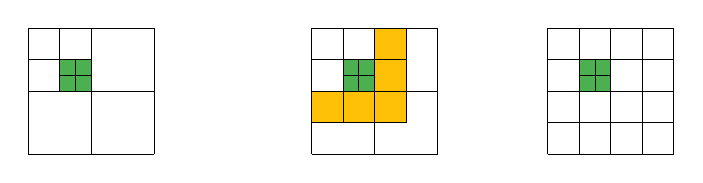
\begin{tikzpicture}[scale=0.2,every node/.style={scale=0.6} ]
\begin{scope}[shift={(22,0)}]
	\draw[step=4] (0,0) grid +(8,8);
	%\draw[step=2] (4,0) grid +(4,4);
	\draw[step=2] (0,4) grid +(4,4);
	%\draw (0,6) grid +(2,2);
	\draw[fill=cpu1](2,4) grid +(2,2) rectangle (2,4);
\end{scope}

\begin{scope}[shift={(40,0)}]
	\draw[step=4] (0,0) grid +(8,8);
	%\draw[step=2] (4,0) grid +(4,4);
	\draw[step=2] (0,4) grid +(4,4);
	%\draw (0,6) grid +(2,2);
	\draw[fill=cpu1] (2,4) grid +(2,2) rectangle (2,4);
	\draw[fill=cpu2] (0,2) rectangle (2,4); 
	\draw[fill=cpu2] (2,2) rectangle (4,4); 
	\draw[fill=cpu2] (4,2) rectangle (6,4); 	
	\draw[fill=cpu2] (4,4) rectangle (6,6);
	\draw[fill=cpu2] (4,6) rectangle (6,8);
\end{scope}

\begin{scope}[shift={(55,0)}]
	\draw[step=4] (0,0) grid +(8,8);
	\draw[step=2] (4,0) grid +(4,4);
	\draw[step=2] (0,4) grid +(4,4);
	\draw[step=2] (0,0) grid +(4,4);
	\draw[step=2] (4,4) grid +(4,4);
	%\draw (0,6) grid +(2,2);
	\draw[fill=cpu1](2,4) grid +(2,2) rectangle (2,4);
\end{scope}

\end{tikzpicture}
\caption{Left most figure shows an octree which violates the 2:1 balanced constraint, where the octants that cause the violation is showed in (\textcolor{cpu1}{$\blacksquare$}). In the middle figure auxiliary balanced octants are showed in (\textcolor{cpu2}{$\blacksquare$}), in other words these are the octants needed to remove the balance constraint violation in (\textcolor{cpu1}{$\blacksquare$}). Right most figure shows the constructed octree with auxiliary balanced octants which satisfies the 2:1 balance constraint. \label{fig:aux_bal}}
\end{figure}

\begin{algorithm}
   \caption{\taux~: The set of auxiliary nodes to balance $\tau_c$}\label{alg::bottom_up}
  \footnotesize
  \begin{algorithmic}[1]
    \Require $\tau_c$ tree on domain $\Omega$
    \Ensure  $t_{aux}$ unique set of auxiliary nodes needed to balance $\tau_c$
	\State $t_{aux} \leftarrow \tau_c$	
    \For  $~e$ in $t_{aux}$
      \State $t_{aux}.add\_unique(N(P(e)))$
    \EndFor
    \State \Return $t_{aux}$
  \end{algorithmic}
\end{algorithm}

\begin{algorithm}
  \caption{\tbal: $2:1$ tree balancing}\label{alg:tree_balance}
  \footnotesize
  \begin{algorithmic}[1]
    \Require An tree $\tau_c$ on domain $\Omega$, starting level $l_1$ and the ending level $l_2$.
    \Ensure $\tau_b$ ordered $2:1$ balanced tree
    \State $K_{oct}\leftarrow 1$
    \State $t_{aux} \leftarrow \taux(t_{cons}) $
	\State $\tau_b \leftarrow \tcons (t_{aux},l_1,l_2,K_{oct})$
	\State \Return $\tau_b$
    %\EndFunction
  \end{algorithmic}
\end{algorithm}

\subsection{Computing the unique node coordinates}
\label{subsec:p_refinement}

In the mesh-free abstraction, the only pertinent information that is stored is the location of the node-coordinates, and hence the location of the nodal basis function. Once the sedectree has been constructed, nodes can be assigned to each sedecant (element) based on the order of the basis functions \cite{kopriva2009}. In order to generate a continuous Galerkin basis, we need to determine a unique set of node coordinates globally, i.e., on shared element faces, edges etc., we have duplicated node coordinates, and these duplicates need to be removed to have the node coordinate associated with a unique element. Additionally, when we have hanging nodes, only the node coordinates corresponding to the larger face/edge will exist, so this removal of node coordinates needs to be done as well. This is done in a single bottom-up traversal of the elements as illustrated in Figure~\ref{fig:cgnodes}. As shown, at each level as we up the tree, we only need to resolve duplicates between the shared faces/edges of siblings, and this is a local operation. All interior nodes can be marked as unique, and so can the interior face nodes once the duplicates including testing for hanging nodes is resolved. Note that hanging nodes will be resolved at the level of the coarser element, so the decision is straightforward to make. At the end of the bottom-up traversal, we have a set of unique node coordinates that is all the information we will store and use for FEM computations. 

\begin{figure}[H]
		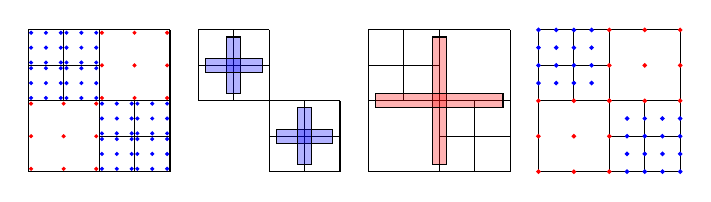
\begin{tikzpicture}[scale=0.18,every node/.style={scale=0.6}]
		
		\begin{scope}[shift={(0,0)}]
		\draw[step=5] (0,0) grid +(10,10);
		\draw[step=2.5] (5,0) grid +(5,5);
		\draw[step=2.5] (0,5) grid +(5,5);
		%\draw[fill=red,fill opacity=0.3] (4.5,0.5) rectangle +(1,9);
		%\draw[fill=red,fill opacity=0.3] (0.5,4.5) rectangle +(9,1);
		%\draw[fill=blue,fill opacity=0.3] (2.0,5.5) rectangle +(1,4);
		%\draw[fill=blue,fill opacity=0.3] (0.5,7.0) rectangle +(4,1);
		%\draw[fill=blue,fill opacity=0.3] (5.5,2.0) rectangle +(4,1);
		%\draw[fill=blue,fill opacity=0.3] (7.0,0.5) rectangle +(1,4);
		%\draw[fill=red!60] (4.2,4.2) circle (0.15);
		
		\def \r{0.1}
		\foreach \x in {0.2,2.5,4.8}{
			\foreach \y in {0.2,2.5,4.8}{
				\draw[red,fill=red] (\x,\y) circle (\r);
			}
		}
		
		\foreach \x in {5.2,7.5,9.8}{
			\foreach \y in {5.2,7.5,9.8}{
				\draw[red,fill=red] (\x,\y) circle (\r);
			}
		}	
		
		\foreach \x in {0.2,1.25,2.3,2.7,3.75,4.8}{
			\foreach \y in {5.2,6.25,7.3}{
				\draw[blue,fill=blue] (\x,\y) circle (\r);
			}
			\foreach \y in {7.7,8.75,9.8}{
				\draw[blue,fill=blue] (\x,\y) circle (\r);
			}  
		}
		
		\foreach \x in {5.2,6.25,7.3,7.7,8.75,9.8}{
			\foreach \y in {0.2,1.25,2.3}{
				\draw[blue,fill=blue] (\x,\y) circle (\r);
			}
			\foreach \y in {2.7,3.75,4.8}{
				\draw[blue,fill=blue] (\x,\y) circle (\r);
			}  
		}
		\end{scope}
		
		\begin{scope}[shift={(12,0)}]
		%\draw[step=5] (0,0) grid +(10,10);
		\draw[step=2.5] (5,0) grid +(5,5);
		\draw[step=2.5] (0,5) grid +(5,5);
		\draw[-] (0,5) -- (5,5);
		\draw[-] (5,0) -- (5,5);
		%\draw[fill=red,fill opacity=0.3] (4.5,0.5) rectangle +(1,9);
		%\draw[fill=red,fill opacity=0.3] (0.5,4.5) rectangle +(9,1);
		\draw[fill=blue,fill opacity=0.3] (2.0,5.5) rectangle +(1,4);
		\draw[fill=blue,fill opacity=0.3] (0.5,7.0) rectangle +(4,1);
		\draw[fill=blue,fill opacity=0.3] (5.5,2.0) rectangle +(4,1);
		\draw[fill=blue,fill opacity=0.3] (7.0,0.5) rectangle +(1,4);
		%\draw[fill=red!60] (4.2,4.2) circle (0.15);
		\end{scope}
		
		
		\begin{scope}[shift={(24,0)}]
		\draw[step=5] (0,0) grid +(10,10);
		\draw[step=2.5] (5,0) grid +(5,5);
		\draw[step=2.5] (0,5) grid +(5,5);
		\draw[fill=red,fill opacity=0.3] (4.5,0.5) rectangle +(1,9);
		\draw[fill=red,fill opacity=0.3] (0.5,4.5) rectangle +(9,1);
		%\draw[fill=blue,fill opacity=0.3] (2.0,5.5) rectangle +(1,4);
		%\draw[fill=blue,fill opacity=0.3] (0.5,7.0) rectangle +(4,1);
		%\draw[fill=blue,fill opacity=0.3] (5.5,2.0) rectangle +(4,1);
		%\draw[fill=blue,fill opacity=0.3] (7.0,0.5) rectangle +(1,4);
		%\draw[fill=red!60] (4.2,4.2) circle (0.15);
		\end{scope}
		
		\begin{scope}[shift={(36,0)}]
        
        \draw[step=5] (0,0) grid +(10,10);
		\draw[step=2.5] (5,0) grid +(5,5);
		\draw[step=2.5] (0,5) grid +(5,5);
		
		\def \r{0.12}
		\foreach \x in {0,2.5,5}{
			\foreach \y in {0,2.5,5}{
				\draw[red,fill=red] (\x,\y) circle (\r);
			}
		}
		
		\foreach \x in {5,7.5,10}{
			\foreach \y in {5,7.5,10}{
				\draw[red,fill=red] (\x,\y) circle (\r);
			}
		}
		
		\foreach \x in {0,1.25,2.5,3.75}{
			\foreach \y in {6.25,7.5,8.75,10}{
				\draw[blue,fill=blue] (\x,\y) circle (\r);
			}
		}	
		
		\foreach \x in {6.25,7.5,8.75,10}{
			\foreach \y in {0,1.25,2.5,3.75}{
				\draw[blue,fill=blue] (\x,\y) circle (\r);
			}
		}
		\end{scope}
		\end{tikzpicture}
		\caption{A simple example of how the cell nodes are placed for quadratic elements in a quadtree. The leftmost figure shows the \textit{locally shared nodes}, which contain duplicates that need to be resolved in order to get \textit{unique shared nodes} (the rightmost figure). We perform a single bottom-up pass of the tree resolving node conflicts, at the corresponding interior region indicated by the same color. 
		\label{fig:cgnodes}}
\end{figure}

\subsection{Efficient SFC-based $kD$-tree traversal}
\label{subsec:treetraverse}
In this section, we present an extension of \tsort~ algorithm to perform efficient traversals on $kD$ trees in order to perform FEM computations. The state-of-the-art approaches\cite{Dendro, mantle, BADER2005994, SundarSampathBiros08} use lookup-tables such as element-to-node mappings, to perform matrix/vector assembly and \mvec. 
%The major drawbacks of these neighborhood data structures include, increasing computational complexity \& memory footprint for higher dimensions and indirect memory accesses lead to bad performances in heterogeneous clusters with deep memory hierarchies. 
In this section, we describe the top-down and bottom-up traversal of the $kD$-tree that are needed for performing these operations without the use of any lookup-tables.
% traversals, which can be top-down, bottom-up or combinations of above, can be used to perform numerical computations which require elemental local nodal values such as FEM computations. 

\textbf{top-down}: In top-down tree traversal for a given non-leaf node $e$, at the corresponding node coordinates, we perform bucketing of the coordinates to the children of $e$, with duplication for the coordinates shared across multiple children (see Figure \ref{fig:traversal}). This process is repeated recursively until we reach a leaf node which can be detected based on the number of coordinates in the bucket. Some buckets might have fewer than the prescribed number of nodes for an element of the specified order. This is because of hanging nodes, and since the nodes of the parent are available at this level, we interpolate these missing values. We recurse in a depth-first fashion as that exposes memory locality and is better suited for deep-memory hierarchies. %Due to the adaptive nature of the tree when we reach a leaf node, some coordinates might be hanging, and those nodal should be able to interpolate from the immediate parent node, due to 2:1 balancing. 

\textbf{bottom-up}: Once we reach a leaf node, we can perform elemental operations ({\em e.g.} elemental \mvec), and if the computation requires an accumulation, nodal values are merged in the reverse direction of the duplication in top-down approach (see \ref{fig:traversal}). 

 \begin{figure}[hbt]
  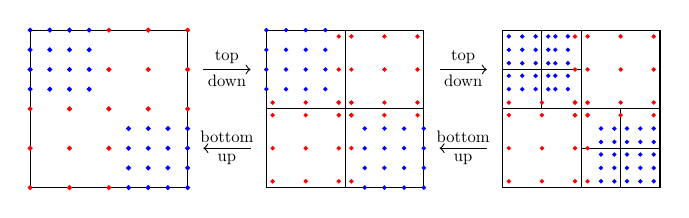
\begin{tikzpicture}[scale=0.2,every node/.style={scale=0.6} ]
	\tikzstyle{edge from parent}=[black,->,shorten <=1pt,>=stealth',semithick,draw]
	\tikzstyle{level 1}=[sibling distance=8mm]
	\tikzstyle{level 2}=[sibling distance=6mm]
	\tikzstyle{level 3}=[sibling distance=4mm]
		
		\begin{scope}[shift={(0,0)}]
		\draw[step=10] (0,0) grid +(10,10);
		%\draw[step=2.5] (5,0) grid +(5,5);
		%\draw[step=2.5] (0,5) grid +(5,5);
		\def \r{0.12}
		\foreach \x in {0,2.5,5}{
			\foreach \y in {0,2.5,5}{
				\draw[red,fill=red] (\x,\y) circle (\r);
			}
		}
		\foreach \x in {5,7.5,10}{
			\foreach \y in {5,7.5,10}{
				\draw[red,fill=red] (\x,\y) circle (\r);
			}
		}
		\foreach \x in {0,1.25,2.5,3.75}{
			\foreach \y in {6.25,7.5,8.75,10}{
				\draw[blue,fill=blue] (\x,\y) circle (\r);
			}
		}	
		\foreach \x in {6.25,7.5,8.75,10}{
			\foreach \y in {0,1.25,2.5,3.75}{
				\draw[blue,fill=blue] (\x,\y) circle (\r);
			}
		}
		\end{scope}
		
		\begin{scope}[shift={(15,0)}]
		\draw[step=5] (0,0) grid +(10,10);
		%\draw[step=2.5] (5,0) grid +(5,5);
		%\draw[step=2.5] (0,5) grid +(5,5);
		\def \r{0.1}
		\foreach \x in {0.4,2.5,4.6,5.4}{
			\foreach \y in {0.4,2.5,4.6,5.4}{
				\draw[red,fill=red] (\x,\y) circle (\r);
			}
		}
		\foreach \x in {4.6,5.4,7.5,9.6}{
			\foreach \y in {4.6,5.4,7.5,9.6}{
				\draw[red,fill=red] (\x,\y) circle (\r);
			}
		}
		\foreach \x in {0,1.25,2.5,3.75}{
			\foreach \y in {6.25,7.5,8.75,10}{
				\draw[blue,fill=blue] (\x,\y) circle (\r);
			}
		}	
		\foreach \x in {6.25,7.5,8.75,10}{
			\foreach \y in {0,1.25,2.5,3.75}{
				\draw[blue,fill=blue] (\x,\y) circle (\r);
			}
		}
		\end{scope}
		
		\begin{scope}[shift={(30,0)}]
		\draw[step=5] (0,0) grid +(10,10);
	    \draw[step=2.5] (5,0) grid +(5,5);
		\draw[step=2.5] (0,5) grid +(5,5);
		\def \r{0.1}
		
		\foreach \x in {0.4,2.5,4.6,5.4}{
			\foreach \y in {0.4,2.5,4.6,5.4}{
				\draw[red,fill=red] (\x,\y) circle (\r);
			}
		}
		\foreach \x in {4.6,5.4,7.5,9.6}{
			\foreach \y in {4.6,5.4,7.5,9.6}{
				\draw[red,fill=red] (\x,\y) circle (\r);
			}
		}
		
		\foreach \x in {0.4,1.25,2.1,2.9,3.35,4.15}{
			\foreach \y in {6.25,7.1,7.9,8.75,9.6}{
				\draw[blue,fill=blue] (\x,\y) circle (\r);
			}
		}	
		\foreach \x in {6.25,7.1,7.9,8.75,9.6}{
			\foreach \y in {0.4,1.25,2.1,2.9,3.75}{
				\draw[blue,fill=blue] (\x,\y) circle (\r);
			}
		}
		
		\end{scope}
		\draw[->] (11,7.5) -- node[above] {top} node[below] {down} (14,7.5);
		\draw[->] (14,2.5) -- node[above] {bottom} node[below] {up} (11,2.5);	
		
		\draw[->] (26,7.5) -- node[above] {top} node[below] {down} (29,7.5);
		\draw[->] (29,2.5) -- node[above] {bottom} node[below] {up} (26,2.5);	
		
		\end{tikzpicture} 
		%\vfill
		
		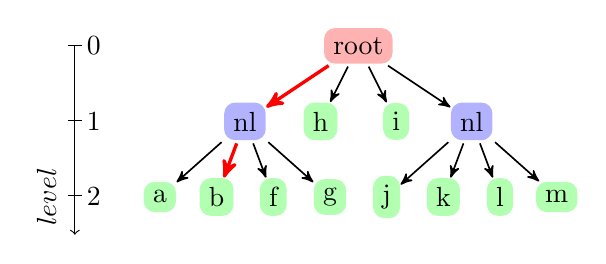
\begin{tikzpicture}[scale=1.2, level distance=8mm,emph/.style={edge from parent/.style={red,->,shorten <=1pt,>=stealth',very thick,draw}},norm/.style={edge from parent/.style={black,->,shorten <=1pt,>=stealth',semithick,draw}}]
    	\tikzstyle{edge from parent}=[black,->,shorten <=1pt,>=stealth',semithick,draw]
    	\tikzstyle{level 1}=[sibling distance=8mm]
    	\tikzstyle{level 2}=[sibling distance=6mm]
    	\tikzstyle{level 3}=[sibling distance=4mm]
    	
    	\node[fill=red!30,rounded corners] {root}
    	child[emph] { node[fill=blue!30,rounded corners] {nl}
    		child[norm] { node[fill=green!30,rounded corners] {a}}
    		child[emph] { node[fill=green!30,rounded corners] {b}
    			%child[norm] { node[fill=green!30,rounded corners] {b}}
    			%child[norm] { node[fill=green!30,rounded corners] {c}}
    			%child[emph] { node[draw=red,very thick,fill=green!30,rounded corners] {d}}
    			%child[norm] { node[fill=green!30,rounded corners] {e}}
    		}
    		child[norm] { node[fill=green!30,rounded corners] {f}}
    		child[norm] { node[fill=green!30,rounded corners] {g}}
    	}
    	child { node[fill=green!30,rounded corners] {h}}
    	child { node[fill=green!30,rounded corners] {i}}
    	child { node[fill=blue!30,rounded corners] {nl}
    		child { node[fill=green!30,rounded corners] {j}}
    		child { node[fill=green!30,rounded corners] {k}}
    		child { node[fill=green!30,rounded corners] {l}}
    		child { node[fill=green!30,rounded corners] {m}}
    	};
    	
    	%% Draw levels axis ...
    	\draw[->] (-3,0) -- (-3,-2);		
    	\draw[snake=ticks,segment length=0.95cm] (-3,0) -- (-3,-2);
    	
    	\draw (-2.8,0) node {$0$}
    	(-2.8,-0.8) node {$1$}
    	(-2.8,-1.6) node {$2$};
    	%(-2.8,-2.4) node {$3$};
    	\draw (-3.3,-1.6) node [rotate=90] {$level$};		
    	%\draw (3,-2.9) node {$\mathcal{R}$};
	
	    \end{tikzpicture}
		
	\caption{Illustration of top-down \& bottom-up tree traversals for a $2D$ tree with quadratic element order. The leftmost figure depicts the unique shared nodes (nodes are color-coded based on level), as we perform top-down traversal nodes shared across children of the parent get duplicated for each bucket recursively, once leaf node is reached it might be missing elemental local nodes, which can be interpolated from immediate parent (see the rightmost figure). After elemental local node computations, bottom-up traversal performed while merging the nodes duplicated in during the top-down traversal.
	    \label{fig:traversal}
	}
\end{figure}

\begin{figure}
    \centering
    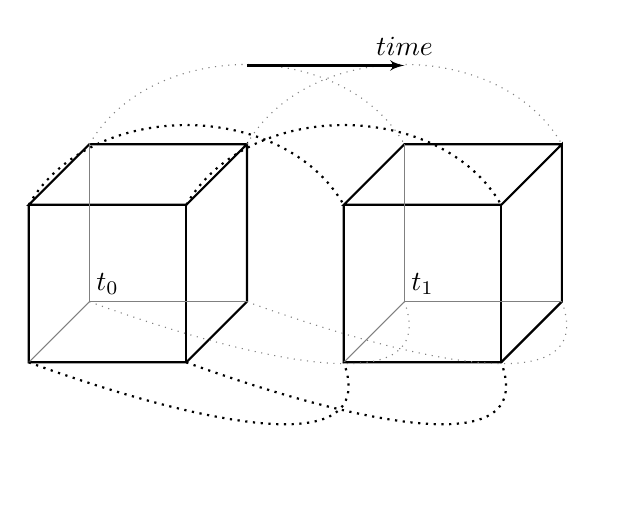
\begin{tikzpicture}
        \draw[thick](2,2,0)--(0,2,0)--(0,2,2)--(2,2,2)--(2,2,0)--(2,0,0)--(2,0,2)--(0,0,2)--(0,2,2);
        \draw[thick](2,2,2)--(2,0,2);
        \draw[gray](2,0,0)--(0,0,0)--(0,2,0);
        \draw[gray](0,0,0)--(0,0,2);
        \draw(1,1,2) node{$t_0$};
        \begin{scope}[shift={(4,0)}]
        \draw[thick](2,2,0)--(0,2,0)--(0,2,2)--(2,2,2)--(2,2,0)--(2,0,0)--(2,0,2)--(0,0,2)--(0,2,2);
        \draw[thick](2,2,2)--(2,0,2);
        \draw[gray](2,0,0)--(0,0,0)--(0,2,0);
        \draw[gray](0,0,0)--(0,0,2);
        \draw(1,1,2) node{$t_1$};
        \end{scope}
        
        \draw[thick,dotted] (2,0,2) to[out=-20,in=-70] (6,0,2);
        \draw[thick,dotted] (0,0,2) to[out=-20,in=-70] (4,0,2);
        
        \draw[gray,dotted] (0,0,0) to[out=-20,in=-70] (4,0,0);
        \draw[gray,dotted] (2,0,0) to[out=-20,in=-70] (6,0,0);
        
        \draw[gray,dotted] (2,2,0) to[out=60,in=120] (6,2,0);
        \draw[gray,dotted] (0,2,0) to[out=60,in=120] (4,2,0);
        
        \draw[thick,dotted] (2,2,2) to[out=60,in=120] (6,2,2);
        \draw[thick,dotted] (0,2,2) to[out=60,in=120] (4,2,2);
        
        \draw[thick, -latex'] (2,3,0) -- (4,3,0) node[above] {$time$};
        
    \end{tikzpicture}
    \caption{Illustration of a \stra. A simple interpretation is that of an octant (in space) represented at two time points, $t_0$ and $t_1$. \label{fig:sedecant}}
\end{figure}

\subsection{Matrix-free implementation on $4D$ meshes}
\label{s:mvec}

As mentioned in the previous section, we will only store the $4D$ coordinates and not any maps (such as element-to-node maps). There are two major reasons for this. Firstly, these maps are very expensive to construct and will have a large memory footprint for $4D$ meshes. Secondly, the variables of interest are accessed and updated using such maps during FEM computations and as such amount to indirect memory access. For large $4D$ meshes in particular, such indirect memory access is likely to be extremely inefficient on modern architectures with high levels of parallelism and deep memory hierarchies. To this effect, we propose a {\em mesh-free} approach that makes use of the quasi-structured nature of \stri s and enables direct access to data. We explain this approach in detail and provide evidence for the efficacy of this approach.  

%For clarity of presentation, we use a simple system system, say corresponding to the heat equation, to explain the $4d$ \mvec. 
We will illustrate a \mvec\ with the transient diffusion operator ($\frac{\partial}{\partial t} + \nabla^2$), given in a discrete form as $K$, i.e., we will compute $v=K u$. Here $u$ is the scalar unknown defined over our spacetime domain, i.e., there is one unknown per node (coordinate point). Therefore the input to our \mvec\ will be the \texttt{real} vector $u$ and another vector of points $\mathbf{p}=(x,y,z,t)$ ($4\times$ \texttt{unsigned int}). The output will be the vector $v$, the same size as $u$ such that $v=K u$. Unlike conventional FEM codes, we will evaluate $v$ without requiring indirect memory accesses to $u,v$ or $\mathbf{p}$. Note that our approach becomes significantly more effective for systems with multiple dofs per spatio-temporal point, as these all will use the same coordinate information. This will be especially useful for both the Navier-Stokes equations (with 4 dofs per point), and the Poisson-Nerst-Plank equations ($n_s+1$ dofs per point, where $n_s$ is the number of species considered).

Since we do not have a mesh, we will have to extract the required information on the fly. Similar to the \stri\ construction, (Figure~\ref{fig:cons}), we proceed in a top-down fashion using the radix sort. This is particularly efficient since we have the $x,y,z$ and $t$ coordinates as \texttt{unsigned int}s. Also, since the coordinates and the unknowns are arranged using space filling curves, there is high locality. In MSD radix, we use the bits--from most to least significant--to bucket the data. In our case, at each level we use one bit each from the $x,y,z$ and $t$ coordinates to bucket the points ($\mathbf{p}$) and unknowns $u$. We then recurse within each bucket. This happens in a depth-first fashion that in combination with the locality of space filling curves, make the overall data-access amenable to modern deep memory hierarchies. Bucketing within radix sort involves only direct memory in a streaming fashion and requires one cache-line for accessing the input and one each for each bucket. 
%Based on the architecture, one can decide to bucket two levels simultaneously ($64$ buckets) using $2$ bits each from $x,y$ and $z$.

\begin{figure}

	 \begin{minted}[frame=lines]{python}
v = {0} 
n = num_non_zero_basis_per_element		
nb = num_buckets;

def matvec(u, x, v, l): # compute v = Ku 
 (U, X, V) = scatter_to_buckets(u, x, v, l)
 for (ui, xi, vi) in (U, X, V):
   if len(xi) == n: # leaf
     for i in [0,n):
       for j in [0,n):
         vi[j] += K_e[i,j] * ui[i];
   else:
     matvec(ui, xi, vi, l-1) # recurse

   gather_from_buckets(vi, x, v, l) 

def U,X = scatter_to_buckets(u, x, l):
 cnt = zeros[nb+1] 
 for _x in x: 
   cnt[_x & (1 << l) + 1]++  
 for (_u, _x) in (u, x):  
   idx = cnt[_x & (1<<l)]++
   U[idx] = _u  
	 X[idx] = _x

def gather_from_buckets(u, x, v, l):
  ... 
  for i in [0,len(x)):  
    idx = cnt[x[i] & (1<<l)]++
    v[i] += u[idx]    
		\end{minted}	
% 	\end{minipage}
	\caption{\label{fig:matvec} \small The pseudocode for the mesh-free $4D$ FEM \texttt{matvec}. Here we compute $v = Ku$ where $u,v$ are specified at coordinates $x,~t$ and $l$ is the level of the \stri, typically $30$. Note that the recursion can terminate early on hitting a leaf node. 
	Note that while access might appear indirect within \texttt{scatter\_to\_bucket} and \texttt{gather\_from\_buckets}, these indices are the bucket numbers and typically small, and $u$ and $v$ are still accessed sequentially, as \texttt{idx} is incremented. 
	While the mesh-free code appears complex, in preliminary tests, %(see Table~\ref{tab:results}), 
	it is approximately $5\times$ faster for scalar PDEs, with the speedup
	increasing for problems with larger dofs.
	}
\end{figure}

Bucketing for the \mvec\ is a bit more involved, so we first illustrate in $2D$ in Figure~\ref{fig:traversal}. Here we need to bucket the interior points and replicate the interior shared faces and the interior corner as well. In $4D$, %Since we bucket recursively, it is sufficient to consider the bucketing from one \stra\ to its children. 
we need to bucket the volumes (faces in 3D) and the interior faces, edges and volumes as these dofs need to be replicated across octants. Once replicated, the \stra s are independent of each other and can recurse independently. This expresses a very fine-grained parallelism not possible with traditional FEM \mvec s. As previously explained, we identify reaching the leaf node based on the when all dofs correspond to the nodes of a single element, potentially with interpolation in case of hanging nodes. Having reached the leaf node, we apply the elemental operator %\footnote{We skip details as either a precomputed elemental matrix or numerical quadrature can be performed and does not affect overall scalability or performance.} 
to compute $v_e = K_e u_e$. On the return, the results in $v$ are accumulated from all children. This is the opposite of the duplication of $u$ prior to the recursion. The simplified pseudocode for the \mvec\ is presented in Figure~\ref{fig:matvec}. 
%For clarity of presentation, we have skipped data-interpolations that are needed by both the traditional as well as mesh-free approaches while working with adaptively refined meshes, such as octrees or \stri s. This does not affect any of the algorithms, and interpolations in both cases happen from parent to child, only when we reach a leaf node. 
%While we have used the recursive formulation for clarity of presentation, the actual implementation uses an iterative variant as that is more efficient. \mf{Is this correct?}

%\hs{data-first, no indirect, fine-grained parallelism.} 
The mesh-free \mvec\ approaches the computation in a data-first fashion and is structured based on the data dependencies and the associated data movement. Note that in the distributed memory setting, we follow a similar principle and exchange ghost or halo regions, albeit using additional lookup tables. Since the mesh-free approach exposes such parallelism in a hierarchical fashion (due to the tree structure), the same basic algorithm holds for the distributed memory cases as well, except that the bucketing at the inter-process level will require {\textsc MPI} communication. Again, unlike traditional codes, this can be done without any additional lookup tables (scatter maps). Also note that the resulting code does not have any indirect memory accesses to the large data arrays $u$ and $v$. This makes implementations simple and easy enough for modern compilers to optimize (such as prefetching, vectorization, etc.) without special architecture specific tuning of the code. 


\section{Results}
\label{sec:Results}
% results goes here. 
\subsection{Experimental Setup:}

The large scalability experiments reported in this paper were
performed on \Titan~and \Stampede. \Titan~is a Cray XK7 supercomputer
at Oak Ridge National Laboratory (ORNL) with a total of 18,688
nodes, each consisting of a single 16-core AMD Opteron 6200 series
processor, with a total of 299,008 cores. Each node has 32GB of memory.
It has a Gemini interconnect and 600TB of memory across all nodes.
%
%\Stampede~ at the Texas Advanced Computing Center (TACC), is a linux cluster consisting of 6400 computes nodes, each with dual, eight-core processors for a total of 102,400 available cpu-cores. Each node has two eight-core 2.7GHz Intel Xeon E5 processors with 2GB/core of memory and a 3 level cache. Stampede has a 56Gb/s FDR Mellanox InfiniBand network connected in a fat tree configuration.
%(In addition, all of Titan's 18,688 compute nodes contain an NVIDIA Tesla K20 graphical processing unit, which we don't use currently). 
%\Stampede~ at the Texas Advanced Computing Center (TACC), is a linux cluster consisting of \textsc{6400} computes nodes, each with dual, eight-core processors for a total of \textsc{102,400} available cpu-cores. Each node has two eight-core 2.7GHz Intel\textsuperscript{\textregistered} Xeon\textsuperscript{\textregistered} E5 processors with 2GB/core of memory and a 3 level cache. Stampede has a \textsc{56Gb/s} FDR Mellanox InfiniBand network connected in a fat tree configuration.
%
\Stampede~  is the flagship supercomputer at the Texas Advanced
Computing Center (TACC), University of Texas at Austin. 
%It has $4,200$ Intel Xeon Phi 7250 (KNL) compute nodes, each with 96GB DDR4 RAM and 16GB of MCDRAM. 
It has $1,736$ Intel Xeon Platinum 8160 (SKX) compute nodes with $2\times 24$ cores and 192GB of RAM
per node. Stampede2 has a 100Gb/sec Intel Omni-Path
(OPA) interconnect in a fat tree topology. We used the SKX
nodes for the experiments reported in this work.


% \begin{figure}
% \hspace{-15 mm}
%     \centering
%     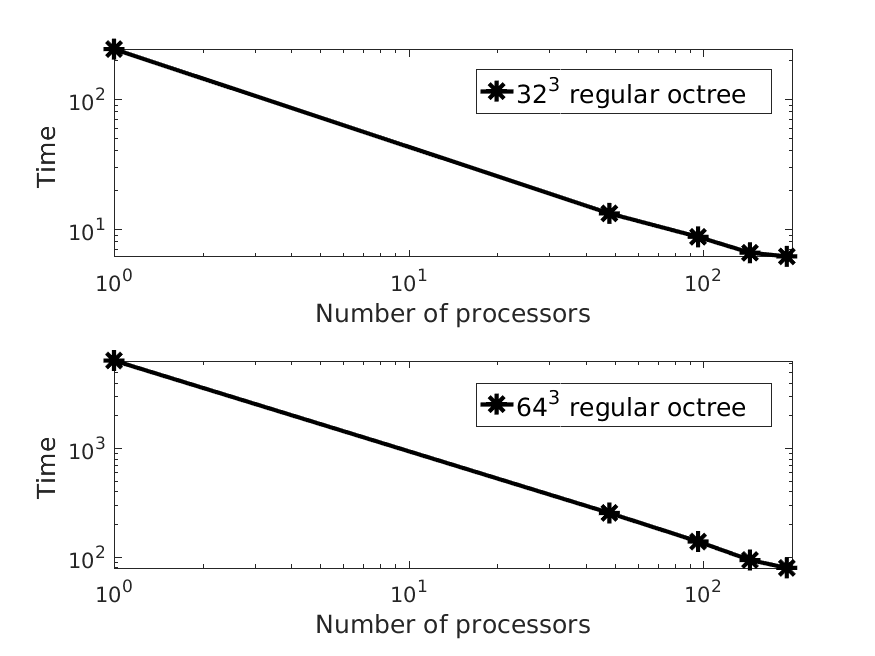
\includegraphics[scale = 0.5]{figs/Rtree.png}
%     \caption{Scaling of 3D + Backward Euler time stepping on TACC \Stampede~ SKX nodes for regular octree using matrix free method. The final time was set to be 1.0 s and the number of time step is equivalent to the number of the points in each direction.}
%     \label{fig:mfree_rtree}
% \end{figure}



\begin{figure}
    \centering
    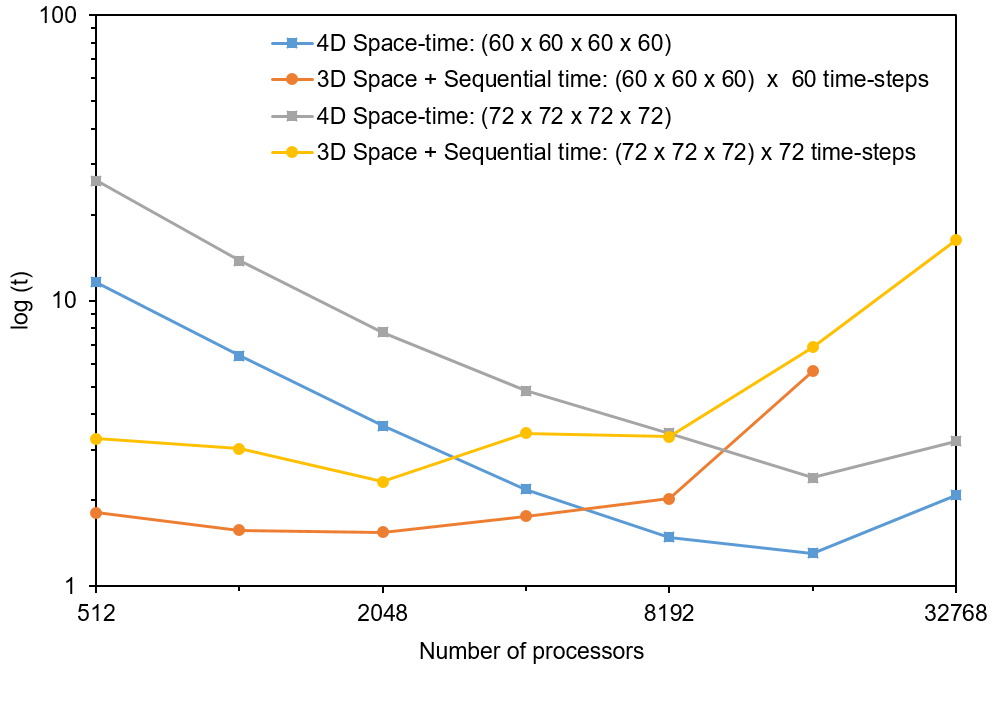
\includegraphics[scale = 0.5]{figs/solve-time-comparison-titan-TS-ST-linear-basis.png}
    \caption{Comparison of scaling of Crank Nicholson time stepping on Titan for linear diffusion problem with coupled space time formulation. The coupled space time formulation scales up to 16384 processors whereas the time stepping scales only up to 2048 processors. }
    \label{fig:comparison_Titan_4D}
\end{figure}

\begin{figure}
    \centering
    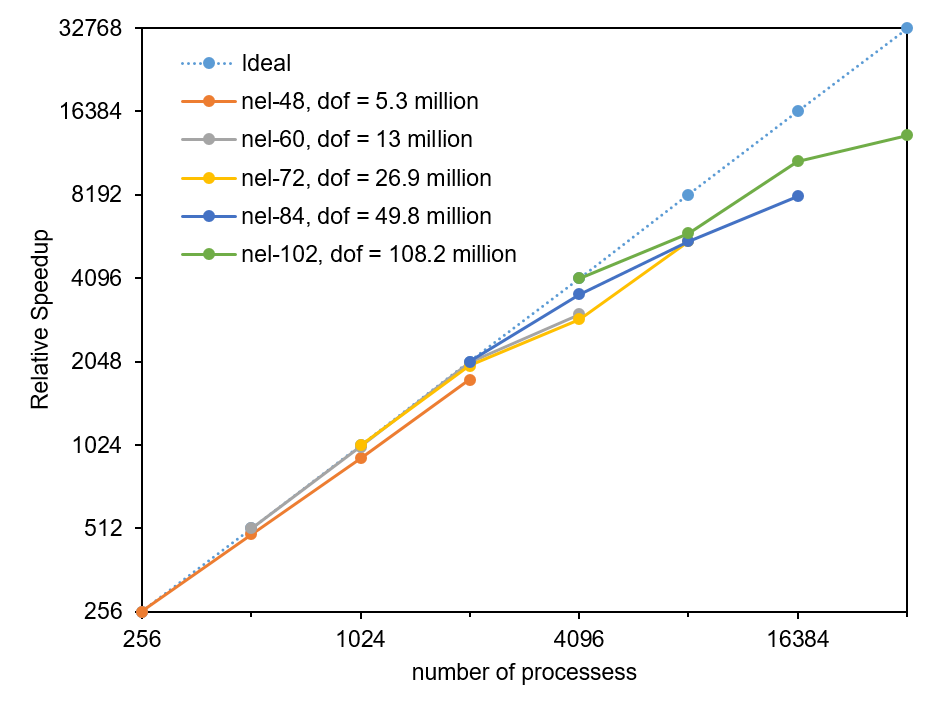
\includegraphics[scale = 0.5]{figs/scaling-titan-LIN-linear-nel-var-speedup.png}
    \caption{Relative speedup  of 4D space - time formulation on Titan. The number of degree of freedom was varied from 5.3 million to 108.2 million across 16384 processors.}
    \label{fig:matrix_Titan_4D}
\end{figure}


%  Then we solve the system using this forcing function (choosing the solution \textit{a priori} also allows us to calculate the analytical error in a suitable norm). %This solution is just an artificial solution chosen in the interest of numerical experimentation and should not be compared with a physically viable solution to the heat equation.
\subsection{Scalability}
We solve the linear diffusion equation \ref{eq:linearheat}, by artificially manufacturing the forcing function, with the given solution $u$ of the form:
\begin{align}\label{def:manufactured-solution}
    u(x, y, z,t) =  e^{t} \sin(\pi x)\sin(\pi y)\sin(\pi z)
\end{align}

Once we have the discrete bilinear form,  the problem is then translated into a linear algebra problem using $4D$ formulation as described in  \S\ref{sec:background} and \S\ref{sec:methodology}. The final linear algebra problem is solved using \petsc~ 3.7 via the \texttt{MATSHELL} interface to expose the mesh-free matrix-free interface. Figure \ref{fig:comparison_Titan_4D} shows the solve time comparison between a time stepping and a space-time problem on \Titan. The time stepping problem solves the PDE \ref{eq:linearheat} in a 3D spatial domain in a prescribed number of time steps through the well known Crank-Nicholson scheme. The space-time counterpart of this problem, is posed in a 4D space-time domain and is solved using the formulation presented in \S\ref{sec:background}. The space-time problem performs badly when the number of processors is low and in this region the time-stepping method is much more efficient. But as the number of processors increase we notice a linear decrease in the solve time for the space-time problem whereas the performance of the time-stepping method deteriorates slowly in the beginning and rapidly when the number of processors go above 5000. This shows concretely the potential of the space-time method with heavy parallelism. By adding the time dimension into the formulation, we are making the problem more complex from the point of view of computation, but this increased complexity in turn allows us to leverage the benefits of high parallelism. Indeed, when number of processors ~ 8000 and above then space-time formulation beats the sequential time stepping solution time.

Figure \ref{fig:matrix_Titan_4D} shows the relative speedup of the 4D space-time problem on  \Titan\ by varying the number of processors from 256 to 32768. The case with 102 elements in each direction (108.2 Million degree of freedom) scales up to 32768 processors. This is a strong scaling result and shows considerably good performance. It must be noted that this %is just the preliminary result with equal elements in each direction of space and time, and 
shows a very high potential to exploit the parallelism on the current scale of machines, which is not possible with the time stepping method. %Both of these cases were computed using the matrix version of the solver. 

We also present strong and weak scaling on \Stampede~ with a breakdown of times for different stages using linear and quadratic basis functions. In Figure \ref{fig:ws_stampede2}, we plot the weak scaling with breakdowns. we observe a dip in the communication costs for the $p=16$ case as this corresponds to a trivial partitioning in the $4D$ case, leading to very low communication costs. The influence on quadratic elements is less pronounced. Our current implementation is not very efficient with memory reuse during the bucketing leading to a significant cost for memory allocations. We are changing this by using a memorypool that should alleviate this problem. Similarly we present strong scaling results in Figure \ref{fig:ss_stampede2}. Again, we see excellent strong scalability for both linear and quadratic basis for a $64\times$ increase in parallelism. 

We are working to get larger runs through the queue on \Titan~ and \Stampede~ and expect even stronger results for larger problems. We expect to have these runs completed before the second round of reviews.
\begin{figure}[tbh]
  \centering
  \begin{tikzpicture}
  \begin{axis}[
  ybar stacked, bar width=5pt,    
  xlabel={number of cores $\rightarrow$},
  ylabel={time(s) $\rightarrow$ },symbolic x coords={2,4,8,16,32,64,128},width=9cm,height=5cm,
  xtick = data, 
  x tick label style={rotate=45, anchor=east, align=right},legend pos=north west,grid=major,ymin=0,ymax=2.5e-4,legend style={at={(0.55,1.0)},
		anchor=south,legend columns=3}]
  \addplot [fill=div_d1] [bar shift=-.125cm] table[x={npes} , y expr={\thisrow{topdown(max)}/(\thisrow{matvecNumNodes}/\thisrow{npes})} ]{dat/stampede2_ws_ele1.dat};
  \addplot [fill=div_d2] [bar shift=-.125cm]  table[x={npes}, y expr={\thisrow{bottomup(max)}/(\thisrow{matvecNumNodes}/\thisrow{npes})} ]{dat/stampede2_ws_ele1.dat};
  \addplot [fill=div_d3] [bar shift=-.125cm]  table[x={npes}, y expr={\thisrow{elemental(max)}/(\thisrow{matvecNumNodes}/\thisrow{npes})} ]{dat/stampede2_ws_ele1.dat};
  \addplot [fill=div_d4] [bar shift=-.125cm]  table[x={npes}, y expr={(\thisrow{matvec(max)}-\thisrow{elemental(max)}-\thisrow{bottomup(max)}-\thisrow{topdown(max)})/(\thisrow{matvecNumNodes}/\thisrow{npes})} ]{dat/stampede2_ws_ele1.dat};
  \addplot [fill=div_d5] [bar shift=-.125cm] table[x={npes}, y expr={\thisrow{ghostexchange(max)}/(\thisrow{matvecNumNodes}/\thisrow{npes})} ]{dat/stampede2_ws_ele1.dat};
  \resetstackedplotsSix
  \addplot [fill=div_d1] [bar shift=+.125cm] table[x={npes} , y expr={\thisrow{topdown(max)}/(\thisrow{matvecNumNodes}/\thisrow{npes})} ]{dat/stampede2_ws_ele2.dat};
  \addplot [fill=div_d2] [bar shift=+.125cm]  table[x={npes}, y expr={\thisrow{bottomup(max)}/(\thisrow{matvecNumNodes}/\thisrow{npes})} ]{dat/stampede2_ws_ele2.dat};
  \addplot [fill=div_d3] [bar shift=+.125cm]  table[x={npes}, y expr={\thisrow{elemental(max)}/(\thisrow{matvecNumNodes}/\thisrow{npes})} ]{dat/stampede2_ws_ele2.dat};
  \addplot [fill=div_d4] [bar shift=+.125cm]  table[x={npes}, y expr={(\thisrow{matvec(max)}-\thisrow{elemental(max)}-\thisrow{bottomup(max)}-\thisrow{topdown(max)})/(\thisrow{matvecNumNodes}/\thisrow{npes})} ]{dat/stampede2_ws_ele2.dat};
  \addplot [fill=div_d5] [bar shift=+.125cm] table[x={npes}, y expr={\thisrow{ghostexchange(max)}/(\thisrow{matvecNumNodes}/\thisrow{npes})} ]{dat/stampede2_ws_ele2.dat};
  \legend{\small top-down, bottom-up, leaf \mvec, malloc, communication}
  \end{axis}
  \begin{axis}[ axis y line=none,axis x line = none,symbolic x coords={2,4,8,16,32,64,128},width=9cm,height=5cm,
        xtick = data,ymin=0,ymax=2.5e-4,legend pos={north west}] %second axis, function 
      \addplot[sq_b1,thin]  table[x={npes}, y expr={(\thisrow{matvec(max)} + \thisrow{ghostexchange(max)}) /(\thisrow{matvecNumNodes}/\thisrow{npes})} ]{dat/stampede2_ws_ele1.dat};
      \addplot[sq_r1,thin,dashed]  table[x={npes}, y expr={(\thisrow{matvec(max)} + \thisrow{ghostexchange(max)}) /(\thisrow{matvecNumNodes}/\thisrow{npes})} ]{dat/stampede2_ws_ele2.dat};
      \legend{linear,quadratic}
  \end{axis}  
 \end{tikzpicture}
\caption{Weak scaling results \textit{mesh-free,matrix-free} FEM \mvec~ on an adaptive $4D$ tree on TACC's Stampede across 128 cores with linear and quadratic basis functions. Note that due to lack of explicit control over the grid size, runtime for the \mvec is reported per degree of freedom per core.}
\label{fig:ws_stampede2}
\end{figure}



\begin{figure}[tbh]
  \centering
  \begin{tikzpicture}
  \begin{axis}[
  ybar stacked, bar width=5pt,    
  xlabel={number of cores $\rightarrow$},
  ylabel={time(s) $\rightarrow$ },symbolic x coords={2,4,8,16,32,64,128},width=9cm,height=5cm,
  xtick = data, 
  x tick label style={rotate=45, anchor=east, align=right},legend pos=north west,grid=major,legend style={at={(0.55,1.0)},
		anchor=south,legend columns=3}]
  \addplot [fill=div_d1] [bar shift=-.125cm] table[x={npes} , y expr={\thisrow{topdown(max)}/\thisrow{matvecNumNodes}} ]{dat/stampede2_ss_ele1.dat};
  \addplot [fill=div_d2] [bar shift=-.125cm]  table[x={npes}, y expr={\thisrow{bottomup(max)}/\thisrow{matvecNumNodes}} ]{dat/stampede2_ss_ele1.dat};
  \addplot [fill=div_d3] [bar shift=-.125cm]  table[x={npes}, y expr={\thisrow{elemental(max)}/\thisrow{matvecNumNodes}} ]{dat/stampede2_ss_ele1.dat};
  \addplot [fill=div_d4] [bar shift=-.125cm]  table[x={npes}, y expr={(\thisrow{matvec(max)}-\thisrow{elemental(max)}-\thisrow{bottomup(max)}-\thisrow{topdown(max)})/\thisrow{matvecNumNodes}} ]{dat/stampede2_ss_ele1.dat};
  \addplot [fill=div_d5] [bar shift=-.125cm] table[x={npes}, y expr={\thisrow{ghostexchange(max)}/\thisrow{matvecNumNodes}} ]{dat/stampede2_ss_ele1.dat};
  \resetstackedplotsSix
  \addplot [fill=div_d1] [bar shift=+.125cm] table[x={npes} , y expr={\thisrow{topdown(max)}/\thisrow{matvecNumNodes}} ]{dat/stampede2_ss_ele2.dat};
  \addplot [fill=div_d2] [bar shift=+.125cm]  table[x={npes}, y expr={\thisrow{bottomup(max)}/\thisrow{matvecNumNodes}} ]{dat/stampede2_ss_ele2.dat};
  \addplot [fill=div_d3] [bar shift=+.125cm]  table[x={npes}, y expr={\thisrow{elemental(max)}/\thisrow{matvecNumNodes}} ]{dat/stampede2_ss_ele2.dat};
  \addplot [fill=div_d4] [bar shift=+.125cm]  table[x={npes}, y expr={(\thisrow{matvec(max)}-\thisrow{elemental(max)}-\thisrow{bottomup(max)}-\thisrow{topdown(max)})/\thisrow{matvecNumNodes}} ]{dat/stampede2_ss_ele2.dat};
  \addplot [fill=div_d5] [bar shift=+.125cm] table[x={npes}, y expr={\thisrow{ghostexchange(max)}/\thisrow{matvecNumNodes}} ]{dat/stampede2_ss_ele2.dat};
  \legend{\small top-down, bottom-up, leaf \mvec, malloc, communication}
  \end{axis}
   \begin{axis}[ axis y line=none,axis x line = none,symbolic x coords={2,4,8,16,32,64,128},width=9cm,height=5cm,
        xtick = data,legend pos={north east}] %second axis, function 
      \addplot[sq_b1,thin]  table[x={npes}, y expr={(\thisrow{matvec(max)} + \thisrow{ghostexchange(max)}) /(\thisrow{matvecNumNodes})} ]{dat/stampede2_ss_ele1.dat};
      \addplot[sq_r1,thin,dashed]  table[x={npes}, y expr={(\thisrow{matvec(max)} + \thisrow{ghostexchange(max)}) /(\thisrow{matvecNumNodes})} ]{dat/stampede2_ss_ele2.dat};
      \legend{linear,quadratic}
  \end{axis}  
  \end{tikzpicture}
 \caption{Strong scaling results for fixed problem size of $2M$ unknowns for \textit{mesh-free,matrix-free} FEM \mvec~ on an adaptive $4D$ tree on TACC's Stampede across 128 cores with linear and quadratic basis functions. Note that due to lack of explicit control over the grid size, runtime for the \mvec is reported per degree of freedom.}
 \label{fig:ss_stampede2}
\end{figure}

\section{Conclusion \& Future Work}
\label{sec:conclusion}
% conclusion goes here. 

In this work we have presented an innovative $4D$ formulation for solving time-dependent PDE problems. We combined this within an adaptive setting and with variable order discretizations to realize a powerful framework. Our choice of algorithms specifically targets modern architectures with deep-memory hierachies and high levels of parallelism. We demonstrated improved strong and weak scaling as a result of the $4D$ formulation that is able to utilize parallel resources more efficiently compared to the traditional $3D$+time approach, where time is treated sequentially. Additionally, we derived both {\it a priori}, as well as residual-based {\it a posteriori} error estimates for the linear time dependent heat diffusion equation, and numerically illustrated improved convergence behavior of the space-time solution approach. By developing sophisticated numerical methods backed by theoretical guarantees of improved convergence, as well as innovative mesh and matrix free algorithms to enable efficient mapping to modern architectures, we have demonstrated impressive scalability results on current supercomputers.
We believe our methods are a first step towards improving the scalability of PDE solvers to the next generation of supercomputers. 

% In the current work, we have shown the enhanced scaling for the coupled space-time compared with the time - stepping method. 

% Further, we would like to exploit the matrix free version to enhance the  scalabilty of the code. Also, we would like to exploit the adaptive refinement in coupled space time based on the \textit{aposteriori} error estimates based on \textit{kD} trees. 

\bibliographystyle{ACM-Reference-Format}
\bibliography{sc19}

\newpage

\section{Artifact Description}
% artifact description goes here. 
\subsection{Getting and Compiling \dendrokt~}

The \dendrokt~ simulation code is freely available at GitHub (link will be disclosed after review process) under the GNU General Public License (GPL). 
The latest version of the code can be obtained by cloning the repository
\begin{lstlisting}[language=bash]
$ git clone https://gitxxx.com/XVI.git
\end{lstlisting}

The following dependencies are required to compile \dendrokt~
\begin{itemize}
	\item C/C++ compilers with C++11 standards and OpenMP support
	\item MPI implementation (e.g. openmpi, mvapich2 )
	\item ZLib compression library (used to write \texttt{.vtu} files in binary format with compression enabled)
	\item BLAS and LAPACK are optional and not needed for current version of \dendrokt~
	\item CMake 2.8 or higher version
\end{itemize}

\textbf{Note}: We have tested the compilation and execution of \dendrokt \ with \texttt{intel}, \texttt{gcc} 4.8 or higher, \texttt{openmpi}, \texttt{mpich2} and \texttt{intelmpi} and \texttt{craympi} (in \Titan) using the linux operating systems. 

To compile the code, execute these commands
\begin{lstlisting}[language=bash]
$ cd <path to XVI directory >
$ mkdir build
$ cd build
$ ccmake ../      
\end{lstlisting}
The following options for \dendrokt~   can then be set in cmake:
\begin{itemize}
	\item \texttt{XVI\_COMPUTE\_CONSTRAINTS} : Enables the computation of Hamiltonian and momentum constraints
	\item \texttt{XVI\_CONSEC\_COMM\_SELECT}  : If \texttt{ON} sub-communicators are selected from consecrative global ranks, otherwise sub-communicators are selected complete binary tree of global ranks (note that in this case global communicator size need to a power of 2).
	\item \texttt{XVI\_ENABLE\_VTU\_CONSTRAINT\_OUT} : Enables constraint variable output while time-stepping 
	\item \texttt{XVI\_ENABLE\_VTU\_OUTPUT} : Enables evolution variable output while time-stepping
	\item \texttt{XVI\_VTK\_BINARY} : If \texttt{ON} vtu files are written in binary format, else ASCII format (binary format recommended).
	\item \texttt{XVI\_VTK\_ZLIB\_COMPRES} : If \texttt{ON} binary format is compressed (only effective if \texttt{XVI\_VTK\_BINARY} is \texttt{ON})
	\item \texttt{HILBERT\_ORDERING} : Hilbert SFC used if \texttt{ON}, otherwise Morton curve is used. (Hilbert curve is recommended to reduce the communication cost.)
	\item \texttt{NUM\_NPES\_THRESHOLD} : When running in large scale set this to $\sqrt{p}$ where $p$ number of mpi tasks for better performance.
	\item \texttt{RK\_SOLVER\_OVERLAP\_COMM\_AND\_COM} : If \texttt{ON} non blocking communication is used and enable overlapping of communication and computation \textit{unzip} (recommended option), otherwise blocking synchronized \textit{unzip} is used.  	
\end{itemize}

After configuring \dendrokt, generate the Makefile (use \texttt{c} to configure and \texttt{g} to generate). Then execute \texttt{make all} to build all the targets.

\subsection{\Stampede~ compute node configuration}
%NUMA node0 CPU(s):     0,2,4,6,8,10,12,14,16,18,20,22,24,26,28,30,32,34,36,38,40,42,44,46,48,50,52,54,56,58,60,62,64,66,68,70,72,74,76,78,80,82,84,86,88,90,92,94
%NUMA node1 CPU(s):     1,3,5,7,9,11,13,15,17,19,21,23,25,27,29,31,33,35,37,39,41,43,45,47,49,51,53,55,57,59,61,63,65,67,69,71,73,75,77,79,81,83,85,87,89,91,93,95
\begin{verbatim}
    TACC_SYSTEM=stampede2
    Architecture:          x86_64
    CPU op-mode(s):        32-bit, 64-bit
    Byte Order:            Little Endian
    CPU(s):                96
    On-line CPU(s) list:   0-95
    Thread(s) per core:    2
    Core(s) per socket:    24
    Socket(s):             2
    NUMA node(s):          2
    Vendor ID:             GenuineIntel
    CPU family:            6
    Model:                 85
    Model name:Intel(R)Xeon(R)
    Platinum 8160 CPU @ 2.10GHz
    Stepping:              4
    CPU MHz:               2100.000
    BogoMIPS:              4200.00
    Virtualization:        VT-x
    L1d cache:             32K
    L1i cache:             32K
    L2 cache:              1024K
    L3 cache:              33792K
    
    MemTotal:       196438176 kB
    MemFree:        191589692 kB
    MemAvailable:   190917852 kB
    Buffers:               0 kB
    Cached:            62136 kB
    SwapCached:            0 kB
    Active:           112696 kB
    Inactive:          39060 kB
    Active(anon):      89860 kB
    Inactive(anon):    10816 kB
    Active(file):      22836 kB
    Inactive(file):    28244 kB
    Unevictable:           0 kB
    Mlocked:               0 kB
    SwapTotal:             0 kB
    SwapFree:              0 kB
    Dirty:                24 kB
    Writeback:             0 kB
    AnonPages:         88792 kB
    Mapped:            34516 kB
    Shmem:             10892 kB
    Slab:            1596960 kB
    SReclaimable:     172696 kB
    SUnreclaim:      1424264 kB
    KernelStack:       23440 kB
    PageTables:         6336 kB
    NFS_Unstable:          0 kB
    Bounce:                0 kB
    WritebackTmp:          0 kB
    CommitLimit:    182687500 kB
    Committed_AS:     475580 kB
    VmallocTotal:   34359738367 kB
    VmallocUsed:     1826376 kB
    VmallocChunk:   34256930848 kB
    HardwareCorrupted:     0 kB
    AnonHugePages:     16384 kB
    CmaTotal:              0 kB
    CmaFree:               0 kB
    HugePages_Total:       0
    HugePages_Free:        0
    HugePages_Rsvd:        0
    HugePages_Surp:        0
    Hugepagesize:       2048 kB
    DirectMap4k:      646976 kB
    DirectMap2M:     8402944 kB
    DirectMap1G:    192937984 kB
\end{verbatim}


\subsection{4D-Hilbert curve}
\label{subsec:4d_hilbert}
A recursive definition of the Hilbert curve specifies a traversal of the unit hypercube in terms of sub-traversals of each child orthant.

The recurrence rule must do two things. It must specify the order in which children are traversed; and it must also specify the orientations of the children's coordinate frames relative to the parent. Depending on these two specifications, various SFCs may be produced. Some of them can be considered valid extensions of the Hilbert curve. Exactly one of them, according to Haverkort, produces an interdimensionally consistent family of extensions to the Hilbert curve.

To set the stage, assume a coordinate system for the unit $K$-cube, with axes numbered $i \in \{0,\dots,K-1\}$ and origin at the center of the $K$-cube. Magnitudes are irrelevant; we are concerned with the signs of coordinates only. We represent a coordinate tuple as a bit string, $x \in \mathbb{B}^K$, where $\mathbb{B} \equiv \{0,1\}$, `1' meaning `+' and `0' meaning `-'. Each child orthant has a unique coordinate string, relative to the parent frame, that, as an integer, is precisely the child number in lexicographic order: $c = \sum_i 2^{x_i}$.

As for the traversal order, the Hilbert curve follows the ``reflected Gray code'' \cite{haverkort2012harmonious}. In our implementation, the $r^\text{th}$ visited child is
\begin{equation*}
  c \leftarrow (r >> 1) \textrm{ XOR } r
\end{equation*}
where ``>{}>'' is the bit-wise right shift operator and ``XOR'' is the bit-wise XOR operator.

The orientation of the $r^\text{th}$ visited child is described by a permutation of, followed by reflections of, the parent coordinate axes. The axis permutation depends on the parity of $r$ and the coloring of axes as $r$ is read as a bit string. Starting from a reverse ordering of axes, if $r$ is even, then even-colored axes are collected in the back, but if $r$ is odd then odd-colored axes are collected in the back. The reflection $m$ of axes (a bit string, `1' meaning reflect) can be defined in terms of $c$ and $r$:
\begin{equation*}
  m \leftarrow ((r-1) >> 1) \textrm{ XOR } (r-1);
\end{equation*}
\begin{equation*}
  m \leftarrow (m \textrm{ AND } -2) \textrm{ OR } ((\textrm{ NOT } c) \textrm{ AND } 1);
\end{equation*}

The above recurrence rule characterizes the SFC relative to a local coordinate frame. The final lookup table must describe the various orientations of the recurrence rule in terms of an absolute coordinate frame.

To generate such a table we define a multiplication operator that transforms the recurrence rule to another coordinate frame, and then we fill out the group closure until all recurrence rules are defined in terms of previously computed recurrence rules. The base case is to take the absolute frame as the local frame, that is, the unmodified definition. The multiplication operator is
\begin{equation*}
  (MA)(ma) = MAm(A^{-1})(A)a = M(AmA^{-1})(Aa)
\end{equation*}
where $a$ and $A$ are axis permutations and $m$ and $M$ are axis reflections.



\end{document}
